\chapter*{Release 2}
\addcontentsline{toc}{chapter}{Release 2}
\markboth{Release 2}{Release 2}
\renewcommand\fbox{\fcolorbox{blue}{white}}
\label{chap:release2}

\section*{Introduction}

Ce chapitre présente la deuxieme version de notre application.Il est composé de quatre sprints qui ont été réalisés en 8 semaines. Nous avons commencé par l'ajout de la fonctionnalité d'authentification a l'aide en utilisant l'OIDC, puis nous avons ajouté la fonctionnalité de gestion de profil, absence et de delegation. Enfin, nous avons ajouté la fonctionnalité de consultation des statistiques. Dans ce chapitre, nous décrirons en détail les fonctionnalités de chaque sprint, les défis que nous avons rencontrés et les solutions que nous avons apportées pour les surmonter.

Release 2 : (Du 3 Avril au 27 Mai 2023)

\fbox{\begin{minipage}{30em}
  \textbf{Organisation des sprints :} \\
  Cette release contient les quatre sprints:
  \begin{itemize}
    \item \textbf{Sprint 5:} Gestion d'authentification OIDC et verification biometrique.
    \item \textbf{Sprint 6:} Gestion du Profil, d'absence et de délégué.
    \item \textbf{Sprint 7:} Consultation des statistique
    \item \textbf{Sprint 8:} .....
  \end{itemize}
\end{minipage}}

\section{Sprint 5 (Gestion d'authentification OIDC et verification biometrique)}

\subsection{Sprint Goal}
Le sprint actuel a pour objectif de présenter une analyse approfondie de l'authentification OIDC et de la vérification biométrique en tant que méthodes d'identification de l'utilisateur.

\subsection{Sprint Backlog}


\begin{adjustwidth}{-1cm}{}
  % \usepackage{longtable}
    
    \begin{longtable}{|c|p{6cm}|c|p{6cm}|c|}
      % \centering
      \hline
      \textbf{ID} & \textbf{User story} & \textbf{ID}  & \textbf{Tâche} & \textbf{Durée} \\
      \hline
      \multirow{2}{*}{1} & En tant que membre scrum , je souhaite me former sur le protocole OIDC. Cette formation doit me permettre de maîtriser les compétences essentielles pour mettre en place une authentification et une autorisation sécurisées dans notre application mobile.
      & 1.1 & Étudier les spécifications techniques d'OIDC pour comprendre comment les implémenter dans notre application mobile. & \multirow{3}{*}{2.5 Jour} \\
      \cline{1-5}
      \multirow{2}{*}{2} & En tant qu'utilisateur, je veux me connecter à l'application Elise Mobile a l'aide d'un compte OIDC. & 2.1 & Développer la fonction qui permet de connecter . &  \multirow{3}{*}{2.5 Jour} \\
      \cline{1-5}
      \multirow{2}{*}{3} & En tant qu'utilisateur, je veux sécuriser les actions sensibles de l'application Elise Mobile en utilisant la vérification biométrique (empreinte digitale, reconnaissance faciale). & 3.1.& Développer la fonctionnalité d'authentification biométrique pour l'empreinte digitale et la reconnaissance faciale. & \multirow{2}{*}{0.5 Jour} \\
      \cline{3-4}
      & & 3.2 & Intégrer les fonctions de vérification biométrique dans certaines actions sensibles tels que la gestion de signature, la signature du document et la gestion des taches. & \\
      \cline{1-5}
  \hline
  \caption{Sprint backlog du Sprint 5}
  \label{tab:sprint-backlog-5}
\end{longtable}
\end{adjustwidth}


\subsection{Implémentation du Sprint 5}
\textbf{•	Diagramme de cas d'utilisation du sprint 5}

% add image
\begin{figure}[H]
  \centering
  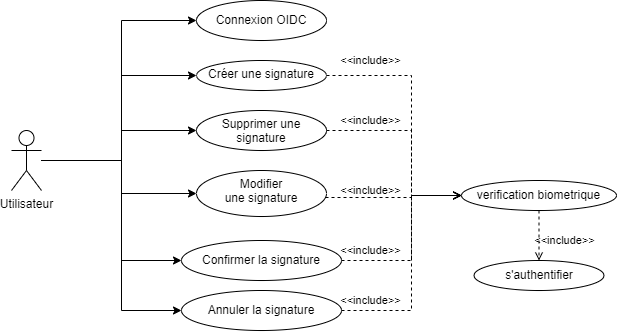
\includegraphics[width=0.8\textwidth]{OIDC_use_case}
  \caption{Diagramme de cas d'utilisation du sprint 5}
  \label{fig:UseCaseDiagramSp51}
\end{figure}

\subsubsection{Analyse des besoins:}
\textbf{•	Description textuelle de cas d'utilisation « Connexion à l'aide du protocole OIDC  »}

\begin{longtable}{|p{5cm}|p{10cm}|}
\hline
\textbf{Cas d'utilisation}&Connexion à l'aide du protocole OIDC\\
\hline
\textbf{Acteurs}&Utilisateur\\
\hline
\textbf{Pré Condition}&L'utilisateur doit avoir un compte OIDC\\
\hline
\textbf{Post Condition}&Authentification\\
\hline
\textbf{Scénario Nominal}&
\vspace{-\baselineskip}
\begin{enumerate}
  \setcounter{enumi}{1}
    \item L'utilisateur saisit le serveur
    \item L'utilisateur clique sur le bouton connexion
    \item Le système vérifie si le serveur existe
    \item Le système affiche la page de login de l'application
    \item L'utilisateur clique sur le bouton « OIDC »
    \item Le système affiche la page login de son serveur d'authentification
    \item L'utilisateur connecte avec son compte
    \item Le système affiche la page de connexion 
    \item Le système vérifie le token
    \item Le système affiche la page d'accueil 
  
\end{enumerate}\\
\hline
\textbf{Scénario alternatif}&
\vspace{-\baselineskip}
\begin{enumerate}
  \item [4.1] Le système affiche le message « le serveur n'existe pas »
  \item [10.1] Le système affiche un message d'erreur
\end{enumerate}\\
\hline
\textbf{Scénario d'exception}&Erreur de connexion\\
\hline
\caption{Description textuelle du diagramme de cas d'utilisation « Consulter les statistiques »}
\label{tab:use_case_oidc_connect}
\end{longtable}

\textbf{•	Description textuelle de cas d'utilisation « Vérification biométrique  »}

\begin{longtable}{|p{5cm}|p{10cm}|}
\hline
\textbf{Cas d'utilisation}&Vérification biométrique \\
\hline
\textbf{Acteurs}&Utilisateur \\
\hline
\textbf{Pré Condition}&
\vspace{-\baselineskip}
\begin{enumerate}
  \setcounter{enumi}{1}
  \item L'utilisateur doit posséder un appareil compatible avec la vérification biométrique
  \item L'utilisateur doit permettre à l'application d'utiliser la vérification biométrique
\end{enumerate}\\
\hline
\textbf{Post Condition}&Vérification biométrique\\
\hline
\textbf{Scénario Nominal}&
\vspace{-\baselineskip}
\begin{enumerate}
    \setcounter{enumi}{1}
    \item L'utilisateur faire l'une des actions sensibles.
    \item Le système vérifie que la dernière date de vérification est supérieure à 5 minutes 
    \item Le système demande une vérification biométrique
    \item L'utilisateur vérifie son identité
    \item Le système vérifie L'identité 
    \item Le système met à jour la date de vérification
    \item Le système exécute L'action
    \item Le système affiche le message de succès
    
\end{enumerate}\\
\hline
\textbf{Scénario alternatif}&
\vspace{-\baselineskip}
\begin{enumerate}
  \item [4.1] Le système passe directement à la 7-ème étape 
  \item [6.1] Le système empêche l'action  
\end{enumerate}\\
\hline
\textbf{Scénario d'exception}&Erreur de connexion\\
\hline
\caption{Description textuelle du diagramme de cas d'utilisation « Consulter les documents a l'aide de filtre rapide »}
\label{tab:use_case_biometric_verification}
\end{longtable}

\begin{figure}[H]
  \centering
  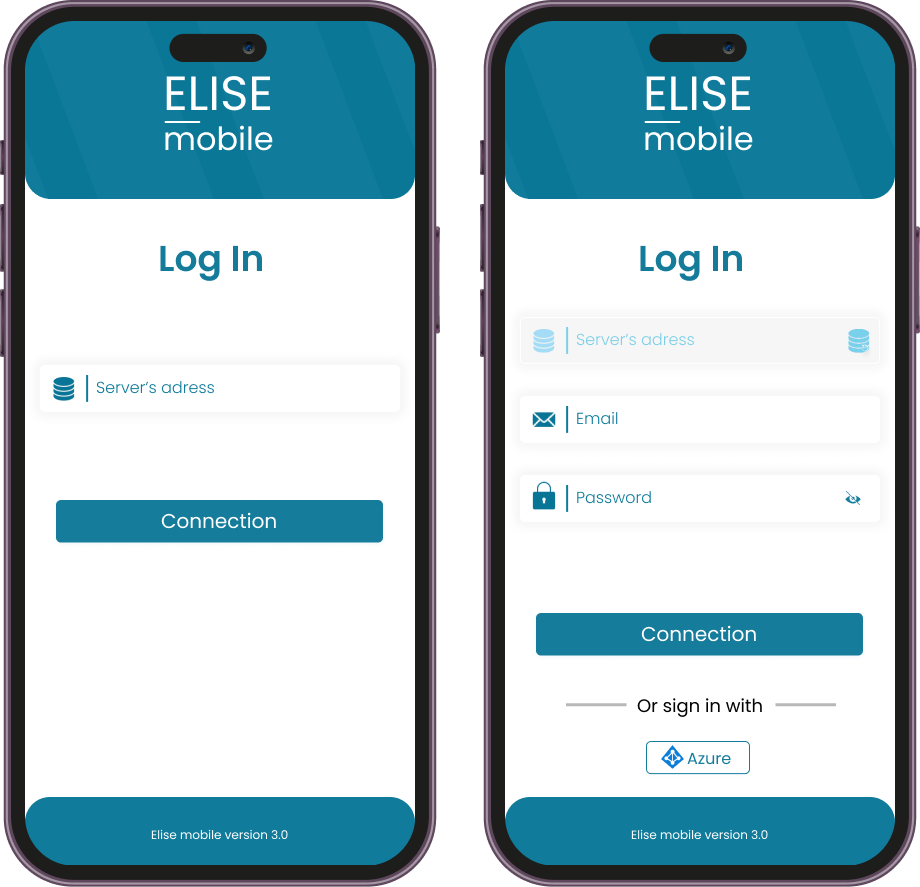
\includegraphics[width=0.7\textwidth]{design_OIDC}
  \caption{Maquette de la page de connexion à l'aide du protocole OIDC}
  \label{fig:design_OIDC}
\end{figure}


Pour avoir une représentation temporelle des interactions entre les objets de notre système et de la chronologie des messages échangés entre eux et avec les acteurs nous avons réalisé les diagrammes de séquence représentés ci-dessous

\begin{figure}[H]
  \centering
  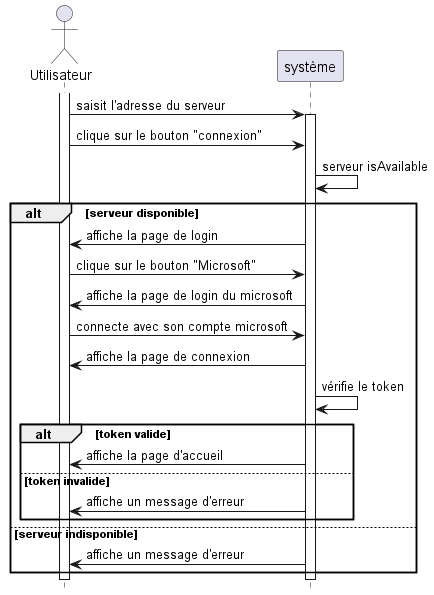
\includegraphics[width=0.7\textwidth]{out/diagrams/sprint5/auth_OIDC/auth_OIDC}
  \caption{Diagramme de séquence de cas d'utilisation « Connexion à l'aide du protocole OIDC »}
  \label{fig:sequence_auth_OIDC}
\end{figure}


\begin{figure}[H]
  \centering
  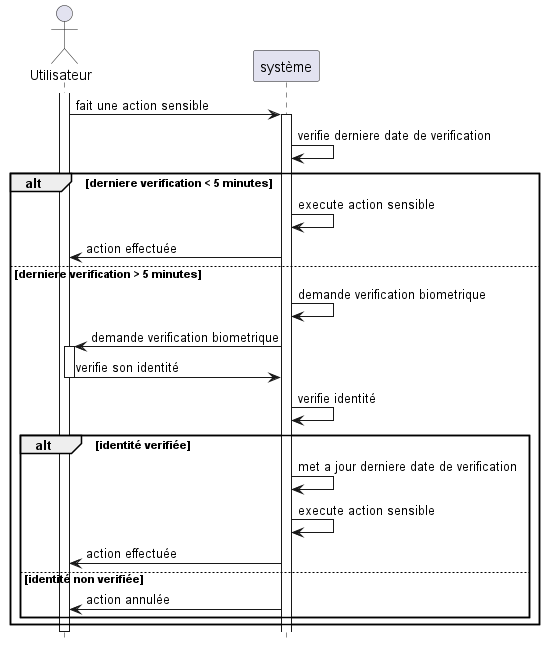
\includegraphics[width=0.7\textwidth]{out/diagrams/sprint5/verification_biometrique/verification_biometrique}
  \caption{Diagramme de séquence de cas d'utilisation « Vérification biométrique »}
  \label{fig:sequence_verification_biometrique}
\end{figure}  
\textbf{Note: C'est un diagramme général qui illustre le processus de vérification biométrique pour différentes actions qui nécessitent une authentification sécurisée, telles que la gestion de signatures, la gestion des tâches et la signature de documents. Ce diagramme montre comment l'utilisateur doit effectuer une vérification biométrique en utilisant des technologies telles que la reconnaissance faciale ou la reconnaissance d'empreintes digitales, pour accéder à des fonctionnalités sensibles de l'application.}


\subsubsection{Analyse détaillée}
La présentation de démarche d'analyse fonctionnelle d'un sprint est très importante pour la satisfaction d'un client parce qu'elle consiste à caractériser les fonctions offertes par un produit.
Donc, nous allons faire l'analyse des différents cas d'utilisation en utilisant le diagramme de classes d'analyse.


% spacing between paragraphs
\setlength{\parskip}{1em}
% spacing left
\setlength{\parindent}{0em}

\textbf{•	Diagramme de classe d'analyse de sprint 5 }


\begin{figure}[H]
  \centering
  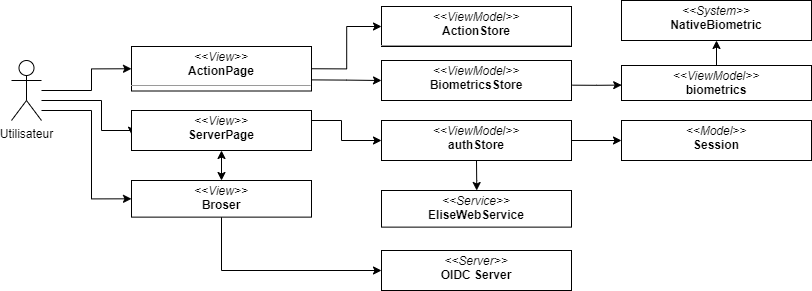
\includegraphics[width=1\textwidth]{dca_sprint5}
  \caption{Diagramme de classe d'analyse de sprint 5}
  \label{fig:class_analyse_sprint5}
\end{figure}


\subsubsection{Conception}

Après la présentation des diagrammes d'analyse, nous avons présenté dans cette partie les diagrammes de conception.\\ 
Nous allons présenter dans cette partie les diagrammes de conception de sprint 5. \\
\textbf{•	Diagramme de classe de conception de sprint 5}

% add image
\begin{figure}[H]
  \centering
  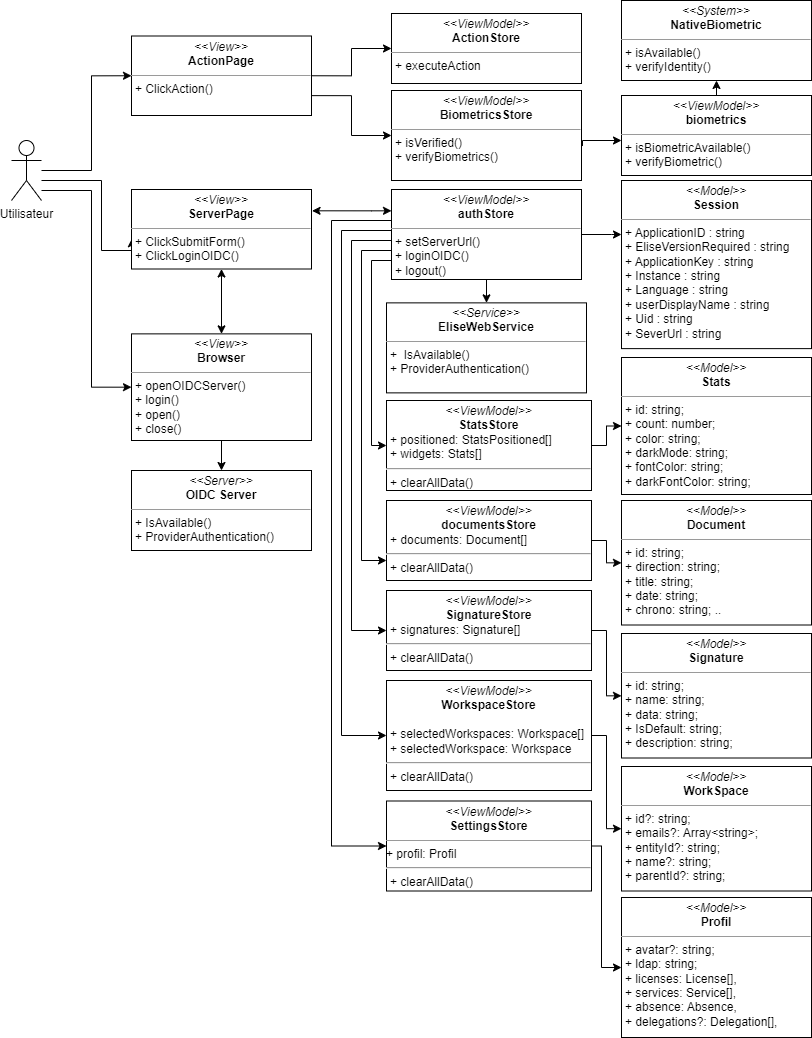
\includegraphics[width=1\textwidth]{dcc_sprint5}
  \caption{Diagramme de classe de conception de sprint 5}
  \label{fig:class_diagram_51}
\end{figure}


\begin{figure}[H]
  \centering
  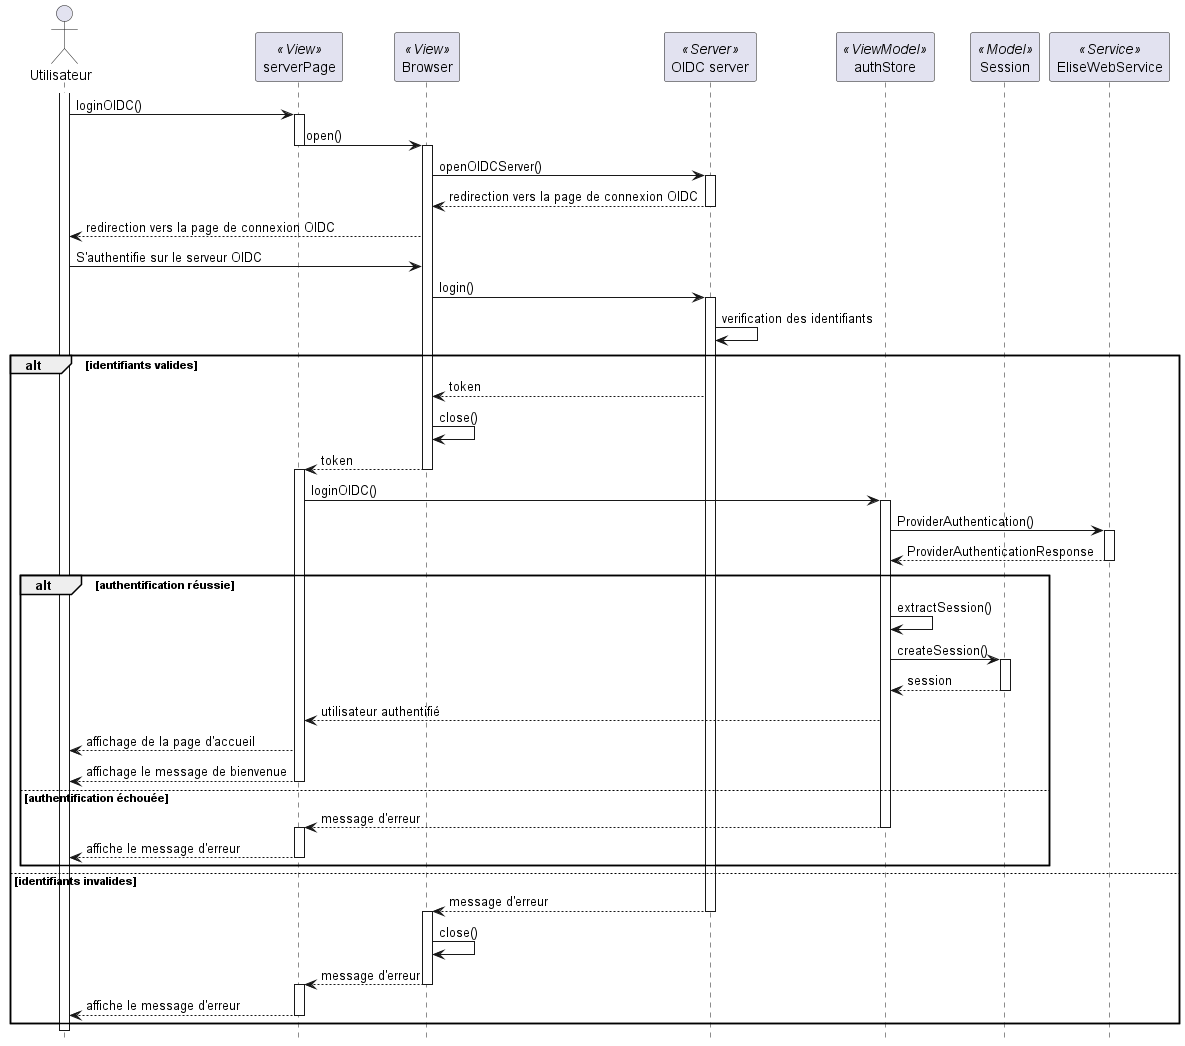
\includegraphics[width=1\textwidth]{out/diagrams/sprint5/sequence_OIDC/sequence_OIDC}
  \caption{Diagramme de séquence de conception de cas d'utilisation « Connexion à l'aide du protocole OIDC »}
  \label{fig:sequence_conception_auth_OIDC}
\end{figure}

\begin{figure}[H]
  \centering
  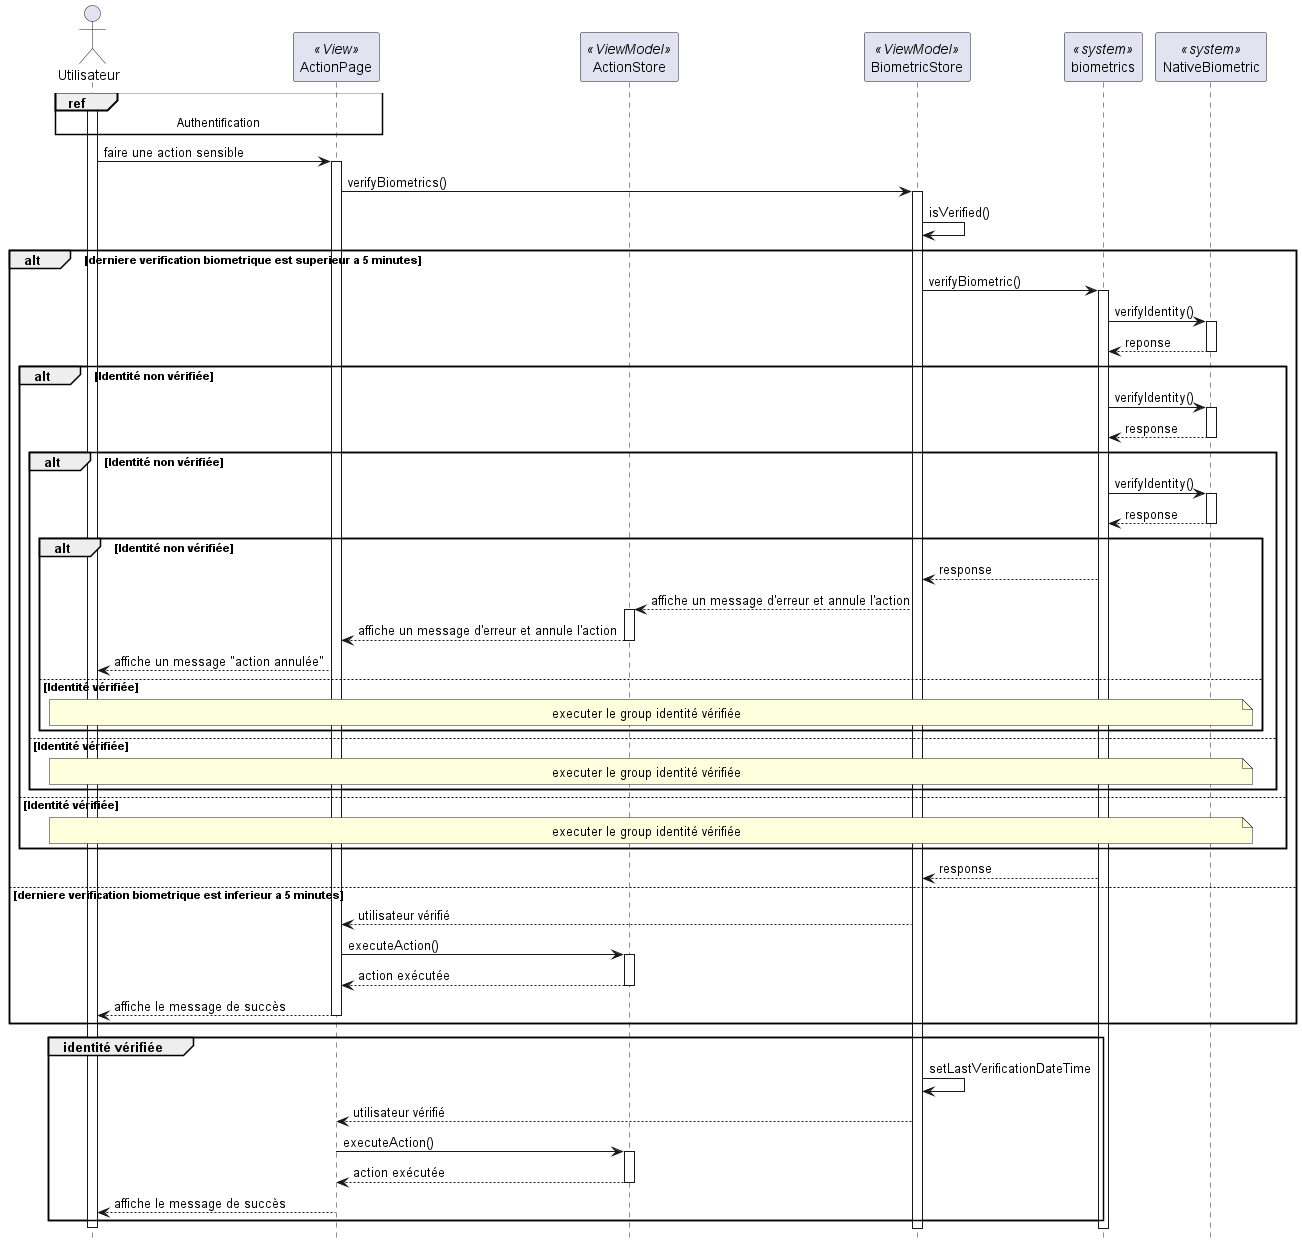
\includegraphics[width=1\textwidth]{out/diagrams/sprint5/sequence_verification_biometrique/sequence_verification_biometrique}
  \caption{Diagramme de séquence de conception de cas d'utilisation « Vérification biométrique »}
  \label{fig:sequence_conception_verification_biometrique}
\end{figure}

\subsubsection{Réalisation}

Après la présentation des diagrammes d'analyse, nous avons présenté dans cette partie des captures d'écran de l'application.

% add image
\begin{figure}[H]
  \centering
  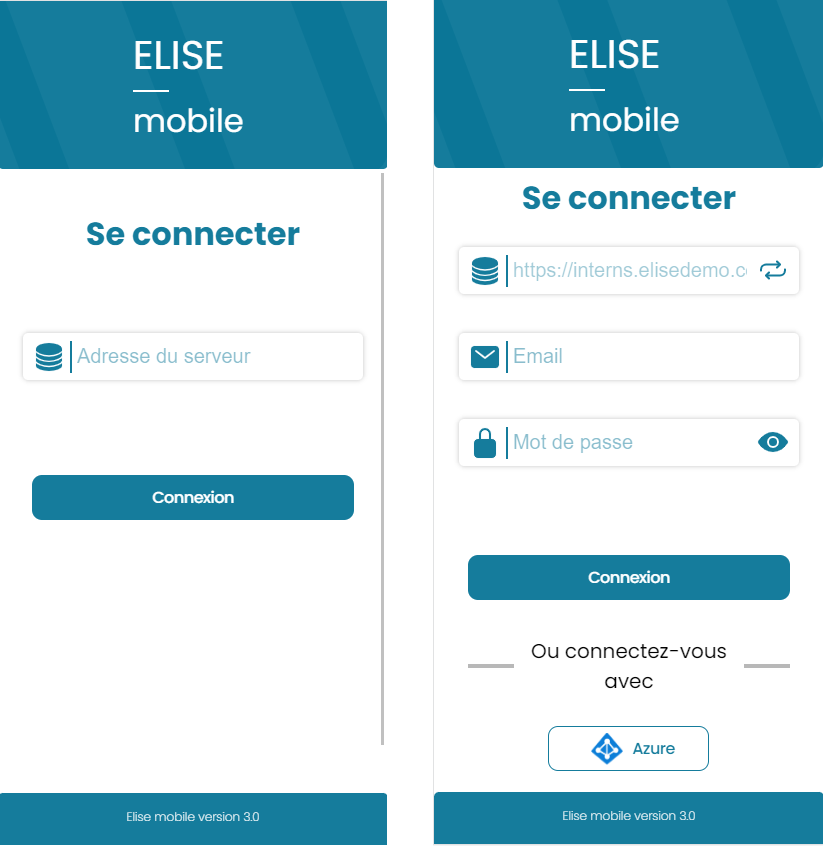
\includegraphics[width=0.7\textwidth, height=0.7\textheight,keepaspectratio=true]{realisation_OIDC}
  \caption{Les interfaces de la page de connexion à l'aide du protocole OIDC}
  \label{fig:realisation_OIDC}
\end{figure}

\subsection{Sprint Review}
Dans ce sprint, nous avons travaillé sur la gestion de l'authentification OIDC et de la vérification biométrique en tant que méthodes d'identification de l'utilisateur.
\subsection{Sprint Retrospective}
Nous avons atteint tous les objectifs fixés pour ce sprint :
\begin{itemize}
  \item \textbf{Ce qui a bien fonctionné :}
  \begin{itemize}
    \item Nous avons produit une analyse complète de l'authentification OIDC et de la vérification biométrique, qui a permis d'identifier les avantages et les limites de chaque méthode d'identification de l'utilisateur.
    \item Offrir une solution plus robuste et plus fiable pour les applications qui requièrent un haut niveau de sécurité.
    
  \end{itemize}

    \item \textbf{Ce qui n'a pas bien fonctionné :}
    \begin{itemize}
      \item Nous avons rencontré des difficultés lors de la mise en œuvre de la fonctionnalité de vérification biométrique et l'authentification OIDC dans l'application Elise Mobile,
    \end{itemize}
      
\end{itemize}
\section{Sprint 6 (Paramétrage des applications et gestion de profil et absence)}

\subsection{Sprint Goal}
Le sprint actuel a pour objectif de gerer les paramétres de l'application, le profil utilisateur, les absences et les délégués en fournissant des fonctionnalités telles que la personnalisation des préférences d'affichage et de notification, la visualisation des informations personnelles, la modification de la photo de profil, la déclaration et l'annulation des absences, la recherche et l'affectation des délégués, ainsi que la suppression des délégués pendant une absence.

\subsection{Sprint Backlog}


\begin{adjustwidth}{-1cm}{}
  % \usepackage{longtable}
    
    \begin{longtable}{|c|p{6cm}|c|p{6cm}|c|}
      % \centering
      \hline
      \textbf{ID} & \textbf{User story} & \textbf{ID}  & \textbf{Tâche} & \textbf{Durée} \\
      \hline
      \multirow{2}{*}{1} & En tant qu'utilisateur, je veux accéder à la page des paramètres afin de personnaliser mon interface et pouvoir accéder a mon profil.
      & 1.1 & Préparer l'interface de paramètres sur Figma. & \multirow{3}{*}{2.5 Jour} \\
      \cline{3-4}
      & & 1.2 & Développer l'interface de paramètres	. & \\
      \cline{1-5}
      \multirow{2}{*}{2} & En tant qu'utilisateur, je veux gérer mes préférences d'affichage de l'application la couleur du thème afin de personnaliser mon application.&2.1&Intégrer la fonctionnalité de mettre à jour les préférences d'affichage de l'utilisateur dans l'application &  \multirow{3}{*}{2.5 Jour} \\
      \cline{1-5}
      \multirow{1}{*}{3} & En tant qu'utilisateur, je souhaite pouvoir choisir la langue de l'application afin de personnaliser mon expérience utilisateur et que l'application se mette automatiquement à jour pour afficher tous les éléments dans la langue sélectionnée. & 3.1 &Intégrer la fonctionnalité de choix de la langue de l'application. & \multirow{1}{*}{0.5 Jour} \\
      \cline{1-5}
      \multirow{1}{*}{4} & En tant qu'utilisateur, je souhaite pouvoir vider le cache de l'application afin d'Améliorer les performances de l'application en supprimant les données stockées dans le cache. & 4.1 &Développer la fonction qui permet de Supprimer le cache. & \multirow{1}{*}{0.5 Jour} \\
      \cline{1-5}
      \multirow{1}{*}{5} & En tant qu'utilisateur, je souhaite pouvoir chercher et sélectionner les espaces de travail afin de consulter les différents documents de chaque espace de travail & 5.1 & Développer la fonction qui permet de récupérer et sélectionner des espaces de travail & \multirow{1}{*}{0.5 Jour} \\
      \cline{1-5}
      \multirow{3}{*}{6} & En tant qu'utilisateur, je veux visualiser mes informations personnelles tels que les services et les licences que je possède pour vérifier leur exactitude et leur actualisation & 6.1 & Préparer l'interface de profil sur Figma & \multirow{3}{*}{2.5 Jour} \\
      \cline{3-4}
      & & 6.2 & Développer l'interface de profil & \\
      \cline{3-4}
      & & 6.3 & Développer la fonction qui permet de récupérer les données & \\
      \cline{1-5}
      \multirow{1}{*}{7} & En tant qu'utilisateur, je veux modifier ma photo de profil pour qu'elle reflète mieux mon image professionnelle ou personnelle actuelle.& 7.1 & Développer la fonction qui permet de modifier mon avatar. & \multirow{1}{*}{0.5 Jour} \\
      \cline{1-5}
      \multirow{3}{*}{8} & En tant qu'utilisateur, je veux déclarer une absence en spécifiant la date de début et la date de fin de mon absence, afin d'informer mes collègues et mes supérieurs hiérarchiques.& 8.1 & Préparer l'interface de gestion d'absence sur Figma & \multirow{3}{*}{2.5 Jour} \\
      \cline{3-4}
      & & 8.2 & Développer l'interface de gestion d'absence & \\
      \cline{3-4}
      & & 8.3 & Développer la fonction qui permet de déclarer une absence & \\
      \cline{1-5}
      \multirow{1}{*}{9} & En tant qu'utilisateur, je veux annuler ma déclaration d'absence si ma situation change et que je suis en mesure de travailler pendant la période initialement déclarée, afin de mettre à jour l'ensemble des parties prenantes informées de mon absence. & 9.1 & Développer la fonction qui permet d'annuler une absence & \multirow{1}{*}{0.5 Jour} \\
      \cline{1-5}
      \multirow{1}{*}{10} & En tant qu'utilisateur, je veux rechercher un utilisateur ou un service et l'affecter comme délégué fin de lui donner les droits nécessaires pour gérer certaines tâches ou projets en mon absence. & 10.1 & Développer la fonction qui permet de d'affecter un utilisateur ou un service comme délégué   & \multirow{1}{*}{0.5 Jour} \\
      \cline{1-5}
      \multirow{1}{*}{11} & En tant qu'utilisateur, je veux supprimer un délégué que j'avais désigné, en cas de besoin ou si je ne suis plus d'accord avec mon choix initial & 11.1 & Développer la fonction qui permet de d'affecter un utilisateur ou un service comme délégué   & \multirow{1}{*}{0.5 Jour} \\
    \hline
  \caption{Sprint backlog du Sprint 6}
  \label{tab:sprint-backlog-6}
\end{longtable}
\end{adjustwidth}


\subsection{Implémentation du Sprint 6}
\textbf{•	Diagramme de cas d'utilisation du sprint 6}

% add image
\begin{figure}[H]
  \centering
  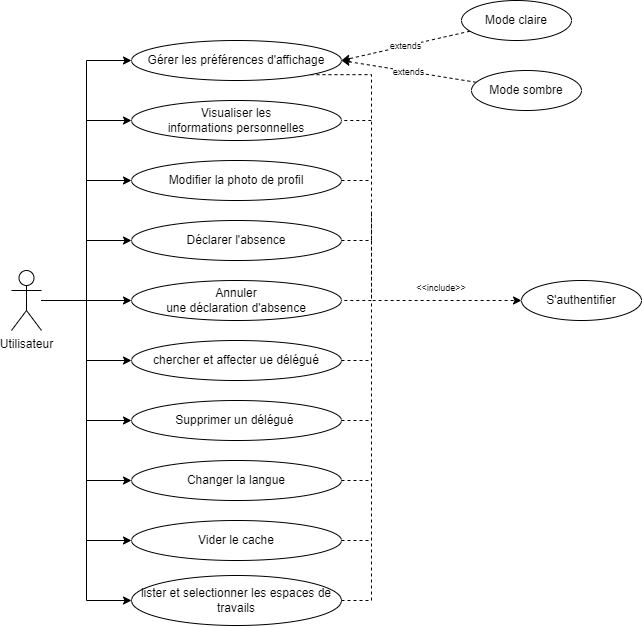
\includegraphics[width=0.7\textwidth]{use_case_sprint_6}
  \caption{Diagramme de cas d'utilisation du sprint 6}
  \label{fig:UseCaseDiagramSp61}
\end{figure}


\subsubsection{Analyse des besoins:}

\textbf{•	Description textuelle de cas d'utilisation « Consulter la page de paramétre  »}

\begin{longtable}{|p{5cm}|p{10cm}|}
\hline
\textbf{Cas d'utilisation}&Consulter la page de paramétre\\
\hline
\textbf{Acteurs}&Utilisateur\\
\hline
\textbf{Pré Condition}&L'utilisateur doit être authentifié\\
\hline
\textbf{Post Condition}&Accès à la page des paramètres\\
\hline
\textbf{Scénario Nominal}&
\vspace{-\baselineskip}
\begin{enumerate}
  \setcounter{enumi}{1}
    \item L'utilisateur clique sur le bouton paramètres.
    \item Le système affiche l'interface de paramètres.
\end{enumerate}\\
\hline
\caption{Description textuelle du diagramme de cas d'utilisation « Consulter la page de paramétre »}
\label{tab:use_case_consult_settings_page}
\end{longtable}


\textbf{•	Description textuelle de cas d'utilisation « Gérer les préférences d'affichage   »}

\begin{longtable}{|p{5cm}|p{10cm}|}
\hline
\textbf{Cas d'utilisation}&Gérer les préférences d'affichage \\
\hline
\textbf{Acteurs}&Utilisateur\\
\hline
\textbf{Pré Condition}&L'utilisateur doit être authentifié\\
\hline
\textbf{Post Condition}&Le thème de l'application est modifié \\
\hline
\textbf{Scénario Nominal}&
\vspace{-\baselineskip}
\begin{enumerate}
  \setcounter{enumi}{1}
 \item L'utilisateur clique sur le bouton thème.
 \item Le système change le thème sombre de l'application.
\end{enumerate}\\
\hline
\textbf{Scénario Alternatif}&
\vspace{-\baselineskip}
\begin{enumerate}
 \item [2.1] Le système change le thème clair de l'application.
\end{enumerate}\\
\hline
\caption{Description textuelle du diagramme de cas d'utilisation « Gérer les préférences d'affichage  »}
\label{tab:use_case_manage_display_preferences}
\end{longtable}

\textbf{•	Description textuelle de cas d'utilisation « Modifier la langue »}

\begin{longtable}{|p{5cm}|p{10cm}|}
\hline
\textbf{Cas d'utilisation}&Modifier la langue \\
\hline
\textbf{Acteurs}&Utilisateur\\
\hline
\textbf{Pré Condition}&L'utilisateur doit être authentifié\\
\hline
\textbf{Post Condition}&La langue de l'application est modifiée \\
\hline
\textbf{Scénario Nominal}&
\vspace{-\baselineskip}
\begin{enumerate}
  \setcounter{enumi}{1}
  \item L'utilisateur clique sur le bouton langues.
  \item Le système affiche le panneau de la liste des langues disponible.
  \item L'utilisateur clique sur la langue souhaitée 
  \item Le système change la langue de l'application
\end{enumerate}\\
\hline
\caption{Description textuelle du diagramme de cas d'utilisation « Modifier la langue  »}
\label{tab:use_case_change_language}
\end{longtable}


\textbf{•	Description textuelle de cas d'utilisation « Vider le cache »}

\begin{longtable}{|p{5cm}|p{10cm}|}
\hline
\textbf{Cas d'utilisation}&Vider le cache  \\
\hline
\textbf{Acteurs}&Utilisateur\\
\hline
\textbf{Pré Condition}&L'utilisateur doit être authentifié\\
\hline
\textbf{Post Condition}&Le cache de l'application est vide \\
\hline
\textbf{Scénario Nominal}&
\vspace{-\baselineskip}
\begin{enumerate}
  \setcounter{enumi}{1}
  \item L'utilisateur clique sur le bouton vider le cache.
  \item Le système affiche le panneau de confirmation contenant la liste des donnés qui vont être supprimer.
  \item L'utilisateur clique sur le bouton confirmer
  \item Le système vide le cache
\end{enumerate}\\
\hline
\textbf{Scénario Alternatif}&
\vspace{-\baselineskip}
\begin{enumerate}
 \item [3.1] L'utilisateur clique sur le bouton annuler
 \item [3.2] Le système annule l'opération
\end{enumerate}\\
\hline
\caption{Description textuelle du diagramme de cas d'utilisation « Vider le cache  »}
\label{tab:use_case_empty_cache}
\end{longtable}


\textbf{•	Description textuelle de cas d'utilisation « chercher et sélectionner un espace de travail  »}

\begin{longtable}{|p{5cm}|p{10cm}|}
\hline
\textbf{Cas d'utilisation}&chercher et sélectionner un espace de travail   \\
\hline
\textbf{Acteurs}&Utilisateur\\
\hline
\textbf{Pré Condition}&L'utilisateur doit être authentifié\\
\hline
\textbf{Post Condition}&Sélectionner des espaces de travails spécifique \\
\hline
\textbf{Scénario Nominal}&
\vspace{-\baselineskip}
\begin{enumerate}
  \setcounter{enumi}{1}
  \item L'utilisateur clique sur le bouton voir espaces de travail.
  \item Le système affiche le panneau de recherche
  \item L'utilisateur saisit le terme de recherche
  \item Le système affiche les espaces de travail contenant le terme de recherche
  \item L'utilisateur clique sur les espaces de travail souhaités
  \item Le système sauvegarde la liste des espaces de travail sélectionnés 
  
\end{enumerate}\\
\hline
\textbf{Scénario Alternatif}&
\vspace{-\baselineskip}
\begin{enumerate}
 \item [4.1] Le système affiche le message « aucun espace de travail trouver » 
\end{enumerate}\\
\hline
\textbf{Scénario d'Exception}&
Erreur de connexion\\
\hline
\caption{Description textuelle du diagramme de cas d'utilisation « chercher et sélectionner un espace de travail   »}
\label{tab:use_case_search_select_workspace}
\end{longtable}


\textbf{•	Description textuelle de cas d'utilisation « Visualiser les informations personnelles  »}

\begin{longtable}{|p{5cm}|p{10cm}|}
\hline
\textbf{Cas d'utilisation}&Visualiser les informations personnelles   \\
\hline
\textbf{Acteurs}&Utilisateur\\
\hline
\textbf{Pré Condition}&L'utilisateur doit être authentifié\\
\hline
\textbf{Post Condition}&Consultation des informations personnelles \\
\hline
\textbf{Scénario Nominal}&
\vspace{-\baselineskip}
\begin{enumerate}
  \setcounter{enumi}{1}
  \item L'utilisateur clique sur le bouton Modifier le Profile.
  \item Le système affiche l'interface de profile.
\end{enumerate}\\
\hline
\textbf{Scénario Alternatif}&
\vspace{-\baselineskip}
\begin{enumerate}
 \item [2.1] Aucun résultat.
\end{enumerate}\\
\hline
\textbf{Scénario d'Exception}&
Erreur de connexion\\
\hline
\caption{Description textuelle du diagramme de cas d'utilisation « Visualiser les informations personnelles   »}
\label{tab:use_case_view_personal_information}
\end{longtable}

\textbf{•	Description textuelle de cas d'utilisation « Modifier la photo de profil  »}

\begin{longtable}{|p{5cm}|p{10cm}|}
\hline
\textbf{Cas d'utilisation}&Modifier la photo de profil   \\
\hline
\textbf{Acteurs}&Utilisateur\\
\hline
\textbf{Pré Condition}&L'utilisateur doit être authentifié\\
\hline
\textbf{Post Condition}&Photo de profil modifié \\
\hline
\textbf{Scénario Nominal}&
\vspace{-\baselineskip}
\begin{enumerate}
  \setcounter{enumi}{1}
  \item L'utilisateur clique sur le bouton camera.
  \item Le système affiche l'interface de camera.
  \item L'utilisateur prend une photo et clique sur le bouton confirmer 
  \item Le système modifie l'avatar de l'utilisateur
\end{enumerate}\\
\hline
\textbf{Scénario Alternatif}&
\vspace{-\baselineskip}
\begin{enumerate}
 \item [3.1] L'utilisateur reprend une autre photo.
\end{enumerate}\\
\hline
\textbf{Scénario d'Exception}&
Erreur de connexion\\
\hline
\caption{Description textuelle du diagramme de cas d'utilisation « Modifier la photo de profil   »}
\label{tab:use_case_modify_profile_picture}
\end{longtable}

\textbf{•	Description textuelle de cas d'utilisation « Déclarer une absence   »}

\begin{longtable}{|p{5cm}|p{10cm}|}
\hline
\textbf{Cas d'utilisation}&Déclarer une absence    \\
\hline
\textbf{Acteurs}&Utilisateur\\
\hline
\textbf{Pré Condition}&L'utilisateur doit être authentifié\\
\hline
\textbf{Post Condition}&Absence déclarée \\
\hline
\textbf{Scénario Nominal}&
\vspace{-\baselineskip}
\begin{enumerate}
  \setcounter{enumi}{1}
  \item L'utilisateur clique sur le bouton activer absence.
  \item Le système déclare l'absence de l'utilisateur.
  
\end{enumerate}\\
\hline
\textbf{Scénario Alternatif}&
\vspace{-\baselineskip}
\begin{enumerate}
 \item [2.1] Aucun résultat.
\end{enumerate}\\
\hline
\textbf{Scénario d'Exception}&
Erreur de connexion\\
\hline
\caption{Description textuelle du diagramme de cas d'utilisation « Déclarer une absence    »}
\label{tab:use_case_declare_absence}
\end{longtable}

\textbf{•	Description textuelle de cas d'utilisation « Annuler une absence    »}

\begin{longtable}{|p{5cm}|p{10cm}|}
\hline
\textbf{Cas d'utilisation}&Annuler une absence     \\
\hline
\textbf{Acteurs}&Utilisateur\\
\hline
\textbf{Pré Condition}&L'utilisateur doit être authentifié\\
\hline
\textbf{Post Condition}&Absence annulée \\
\hline
\textbf{Scénario Nominal}&
\vspace{-\baselineskip}
\begin{enumerate}
  \setcounter{enumi}{1}
  \item L'utilisateur clique sur le bouton désactiver absence.
  \item Le système désactive l'absence de l'utilisateur.
\end{enumerate}\\
\hline
\textbf{Scénario Alternatif}&
\vspace{-\baselineskip}
\begin{enumerate}
 \item [2.1] Aucun résultat.
\end{enumerate}\\
\hline
\textbf{Scénario d'Exception}&
Erreur de connexion\\
\hline
\caption{Description textuelle du diagramme de cas d'utilisation « Annuler une absence     »}
\label{tab:use_case_cancel_absence}
\end{longtable}


\textbf{•	Description textuelle de cas d'utilisation « Chercher et affecter un délégué     »}

\begin{longtable}{|p{5cm}|p{10cm}|}
\hline
\textbf{Cas d'utilisation}&Chercher et affecter un délégué      \\
\hline
\textbf{Acteurs}&Utilisateur\\
\hline
\textbf{Pré Condition}&L'utilisateur doit être authentifié\\
\hline
\textbf{Post Condition}&Affectation d'un délégué \\
\hline
\textbf{Scénario Nominal}&
\vspace{-\baselineskip}
\begin{enumerate}
  \setcounter{enumi}{1}
  \item L'utilisateur clique sur le bouton ajouter.
  \item Le système affiche le panneau de création.
  \item l'utilisateur saisit le terme de recherche
  \item Le système affiche les services / utilisateurs qui correspond aux termes de recherches
  \item L'utilisateur clique sur le service / utilisateur souhaiter et clique sur confirmer 
  \item Le système ajoute le délégué 
\end{enumerate}\\
\hline
\textbf{Scénario Alternatif}&
\vspace{-\baselineskip}
\begin{enumerate}
 \item [4.1] le Système affiche le message « aucun résultat trouvé » 
\end{enumerate}\\
\hline
\textbf{Scénario d'Exception}&
Erreur de connexion\\
\hline
\caption{Description textuelle du diagramme de cas d'utilisation « Chercher et affecter un délégué      »}
\label{tab:use_case_search_delegate}
\end{longtable}


\textbf{•	Description textuelle de cas d'utilisation « Annuler une Délégation      »}

\begin{longtable}{|p{5cm}|p{10cm}|}
\hline
\textbf{Cas d'utilisation}&Annuler une Délégation       \\
\hline
\textbf{Acteurs}&Utilisateur\\
\hline
\textbf{Pré Condition}&L'utilisateur doit être authentifié\\
\hline
\textbf{Post Condition}&Absence annulée \\
\hline
\textbf{Scénario Nominal}&
\vspace{-\baselineskip}
\begin{enumerate}
  \setcounter{enumi}{1}
  \item L'utilisateur clique sur le bouton supprimer.
  \item Le système affiche le panneau de confirmation.
  \item L'utilisateur clique sur le bouton confirmer
  \item Le système supprime la délégation 
\end{enumerate}\\
\hline
\textbf{Scénario Alternatif}&
\vspace{-\baselineskip}
\begin{enumerate}
  \item [3.1]- L'utilisateur clique sur le bouton annuler
  \item [3.2]- aucun traitement
\end{enumerate}\\
\hline
\textbf{Scénario d'Exception}&
Erreur de connexion\\
\hline
\caption{Description textuelle du diagramme de cas d'utilisation « Annuler une Délégation       »}
\label{tab:use_case_cancel_delegate}
\end{longtable}

\begin{figure}[H]
  \centering
  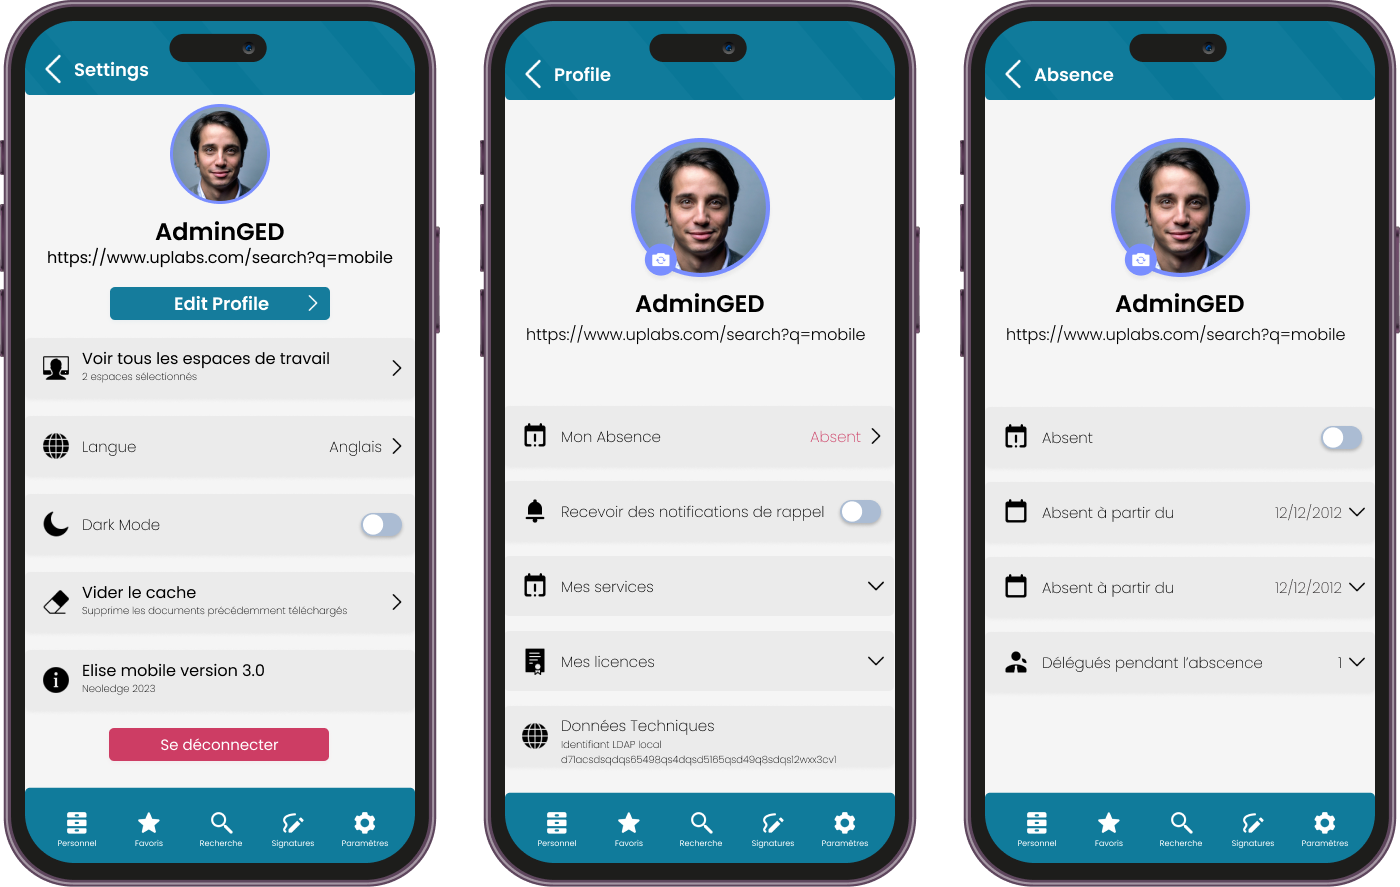
\includegraphics[width=0.7\textwidth]{design_sprint_6}
  \caption{Maquette de l'interface de paramétrage et de gestion des absences}
  \label{fig:MaquetteInterfaceParametrageGestionAbsences}
\end{figure}


Pour avoir une représentation temporelle des interactions entre les objets de notre système et de la chronologie des messages échangés entre eux et avec les acteurs nous avons réalisé les diagrammes de séquence représentés ci-dessous

\begin{figure}[H]
  \centering
  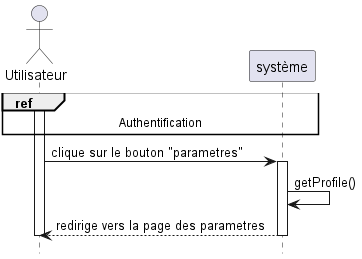
\includegraphics[width=0.7\textwidth]{out/diagrams/sprint6/consult_settings_page/consult_settings_page}
  \caption{Diagramme de séquence de cas d'utilisation « Consulter la page de paramétre »}
  \label{fig:sequence_consult_settings_page}
\end{figure}

\begin{figure}[H]
  \centering
  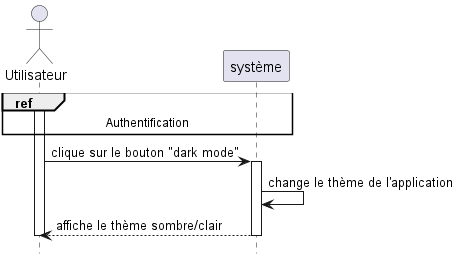
\includegraphics[width=0.7\textwidth]{out/diagrams/sprint6/preferance_affichage/preferance_affichage}
  \caption{Diagramme de séquence de cas d'utilisation « Gérer les préférences d'affichage »}
  \label{fig:sequence_preference_affichage}
\end{figure}


\begin{figure}[H]
  \centering
  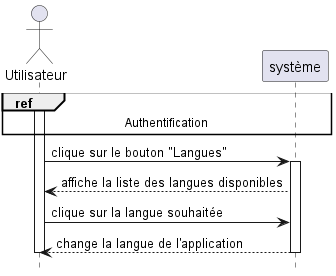
\includegraphics[width=0.7\textwidth]{out/diagrams/sprint6/change_language/change_language}
  \caption{Diagramme de séquence de cas d'utilisation « Changer la langue »}
  \label{fig:sequence_change_language}
\end{figure}

\begin{figure}[H]
  \centering
  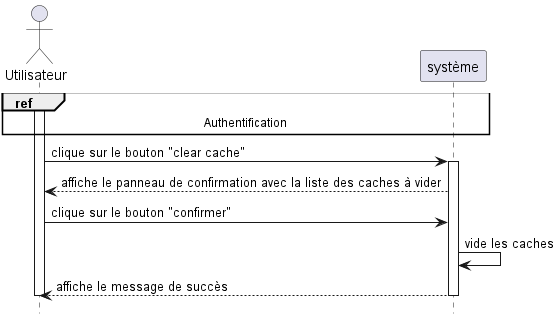
\includegraphics[width=0.7\textwidth]{out/diagrams/sprint6/clear_cache/clear_cache}
  \caption{Diagramme de séquence de cas d'utilisation « Vider le cache »}
  \label{fig:sequence_clear_cache}
\end{figure}

\begin{figure}[H]
  \centering
  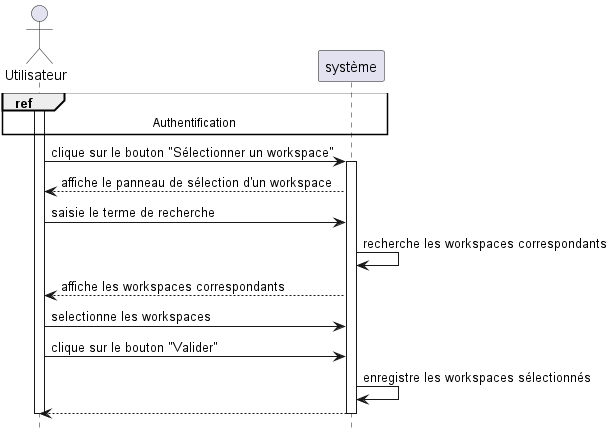
\includegraphics[width=0.7\textwidth]{out/diagrams/sprint6/lister_selectionner_workspaces/lister_selectionner_workspaces}
  \caption{Diagramme de séquence de cas d'utilisation « Lister et sélectionner les espaces de travail »}
  \label{fig:sequence_lister_selectionner_workspaces}
\end{figure}

\begin{figure}[H]
  \centering
  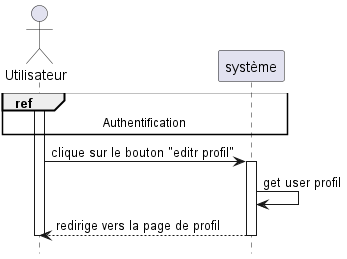
\includegraphics[width=0.7\textwidth]{out/diagrams/sprint6/visualiser_profil/visualiser_profil}
  \caption{Diagramme de séquence de cas d'utilisation « Visualiser les informations personnelles »}
  \label{fig:sequence_visualiser_profil}
\end{figure}

\begin{figure}[H]
  \centering
  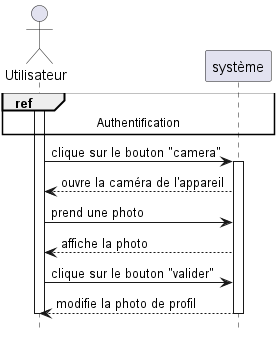
\includegraphics[width=0.7\textwidth]{out/diagrams/sprint6/edit_profil_avatar/edit_profil_avatar}
  \caption{Diagramme de séquence de cas d'utilisation « Modifier la photo de profil »}
  \label{fig:sequence_edit_profil_avatar}
\end{figure}

\begin{figure}[H]
  \centering
  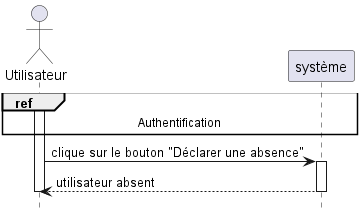
\includegraphics[width=0.7\textwidth]{out/diagrams/sprint6/declare_absence/declare_absence}
  \caption{Diagramme de séquence de cas d'utilisation « Déclarer l'absence »}
  \label{fig:sequence_declare_absence}
\end{figure}

\begin{figure}[H]
  \centering
  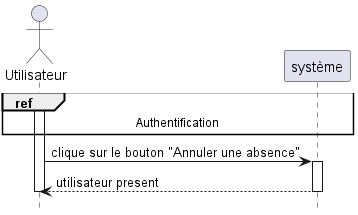
\includegraphics[width=0.7\textwidth]{out/diagrams/sprint6/annuler_absence/annuler_absence}
  \caption{Diagramme de séquence de cas d'utilisation « Annuler une déclaration d'absence »}
  \label{fig:sequence_annuler_absence}
\end{figure}

\begin{figure}[H]
  \centering
  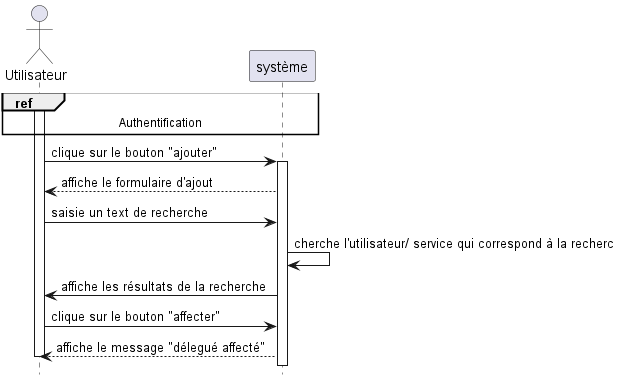
\includegraphics[width=0.7\textwidth]{out/diagrams/sprint6/search_affect_delegation/search_affect_delegation}
  \caption{Diagramme de séquence de cas d'utilisation « Rechercher et affecter un délégué »}
  \label{fig:sequence_search_affect_delegation}
\end{figure}

\begin{figure}[H]
  \centering
  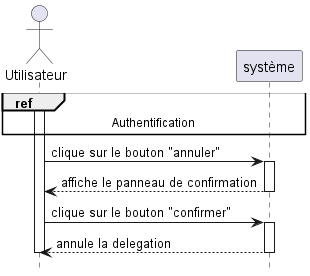
\includegraphics[width=0.7\textwidth]{out/diagrams/sprint6/annulation_delegation/annulation_delegation}
  \caption{Diagramme de séquence de cas d'utilisation « Supprimer un délégué »}
  \label{fig:sequence_annulation_delegation}
\end{figure}




\subsubsection{Analyse détaillée}
La présentation de démarche d'analyse fonctionnelle d'un sprint est très importante pour la satisfaction d'un client parce qu'elle consiste à caractériser les fonctions offertes par un produit.
Donc, nous allons faire l'analyse des différents cas d'utilisation en utilisant le diagramme de classes d'analyse.


% spacing between paragraphs
\setlength{\parskip}{1em}
% spacing left
\setlength{\parindent}{0em}

\textbf{•	Diagramme de classe d'analyse de sprint 6 }


\begin{figure}[H]
  \centering
  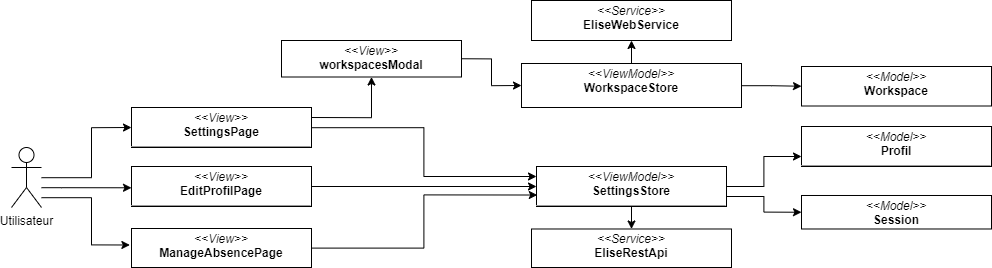
\includegraphics[width=0.9\textwidth]{dca_sprint6}
  \caption{Diagramme de classe d'analyse de sprint 6}
  \label{fig:class_analyse_sprint6}
\end{figure}


\subsubsection{Conception}

Après la présentation des diagrammes d'analyse, nous avons présenté dans cette partie les diagrammes de conception.\\ 
Nous allons présenter dans cette partie les diagrammes de conception de sprint 6. 
\begin{landscape}

\textbf{•	Diagramme de classe de conception de sprint 6}

\begin{figure}[H]
  \centering
  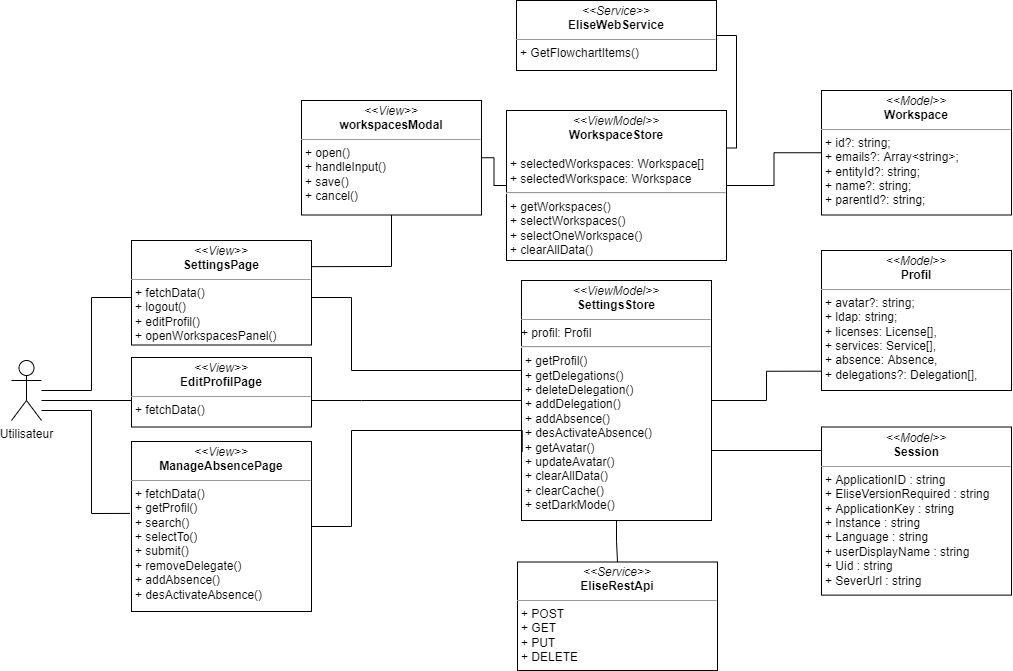
\includegraphics[width=\paperwidth]{dcc_sprint6}
  \caption{Diagramme de classe de conception de sprint 6}
  \label{fig:class_diagram_61}
\end{figure}
\end{landscape}


\begin{figure}[H]
  \centering
  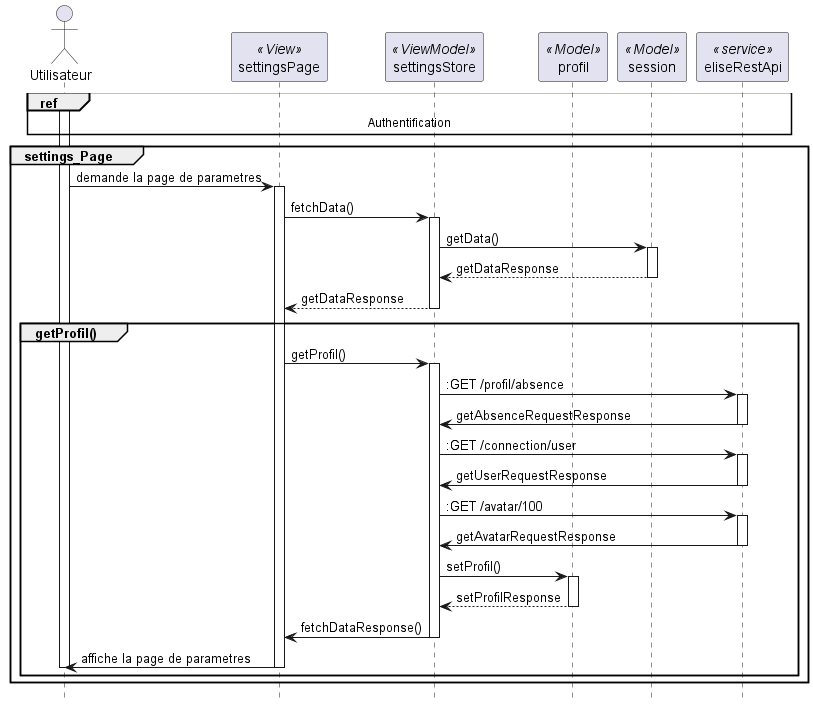
\includegraphics[width=1\textwidth]{out/diagrams/sprint6/sequence_consult_settings_page/sequence_consult_settings_page}
  \caption{Diagramme de séquence de conception de cas d'utilisation « Consulter la page de paramétre »}
  \label{fig:conception_sequence_consult_settings_page}
\end{figure}

\begin{figure}[H]
  \centering
  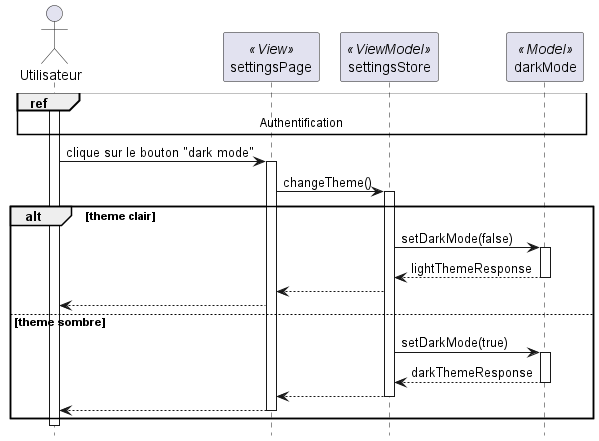
\includegraphics[width=1\textwidth]{out/diagrams/sprint6/sequence_preferance_affichage/sequence_preferance_affichage}
  \caption{Diagramme de séquence de conception de cas d'utilisation « Gérer les préférences d'affichage»}
  \label{fig:conception_sequence_preferance_affichage}
\end{figure}

\begin{figure}[H]
  \centering
  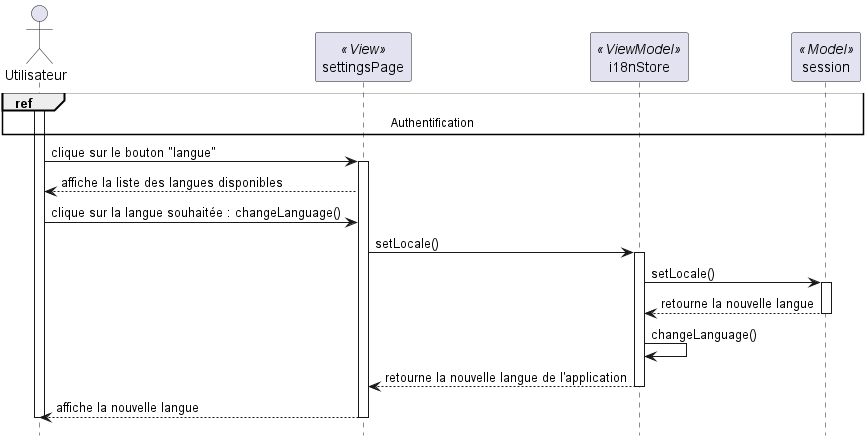
\includegraphics[width=1\textwidth]{out/diagrams/sprint6/sequence_change_language/sequence_change_language}
  \caption{Diagramme de séquence de conception de cas d'utilisation «Changer la langue »}
  \label{fig:conception_sequence_change_language}
\end{figure}

\begin{figure}[H]
  \centering
  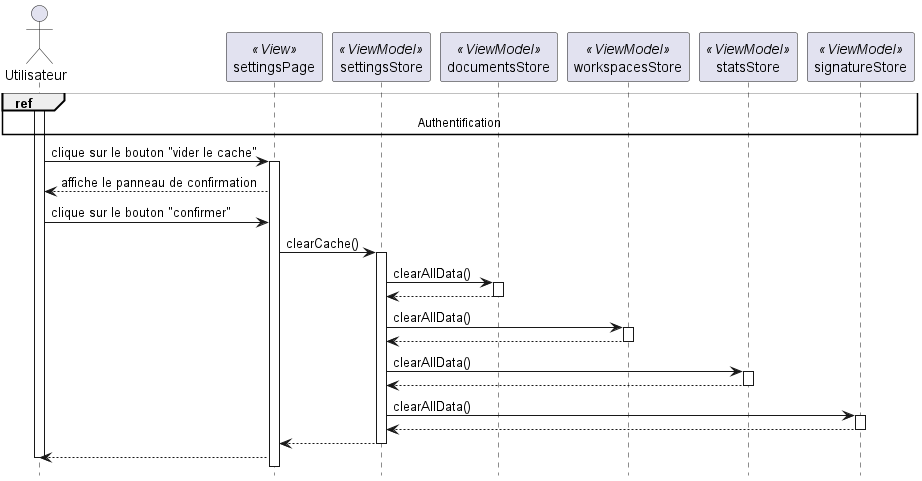
\includegraphics[width=1\textwidth]{out/diagrams/sprint6/sequence_clear_cache/sequence_clear_cache}
  \caption{Diagramme de séquence de conception de cas d'utilisation «  Vider le cache »}
  \label{fig:conception_sequence_clear_cache}
\end{figure}

\begin{figure}[H]
  \centering
  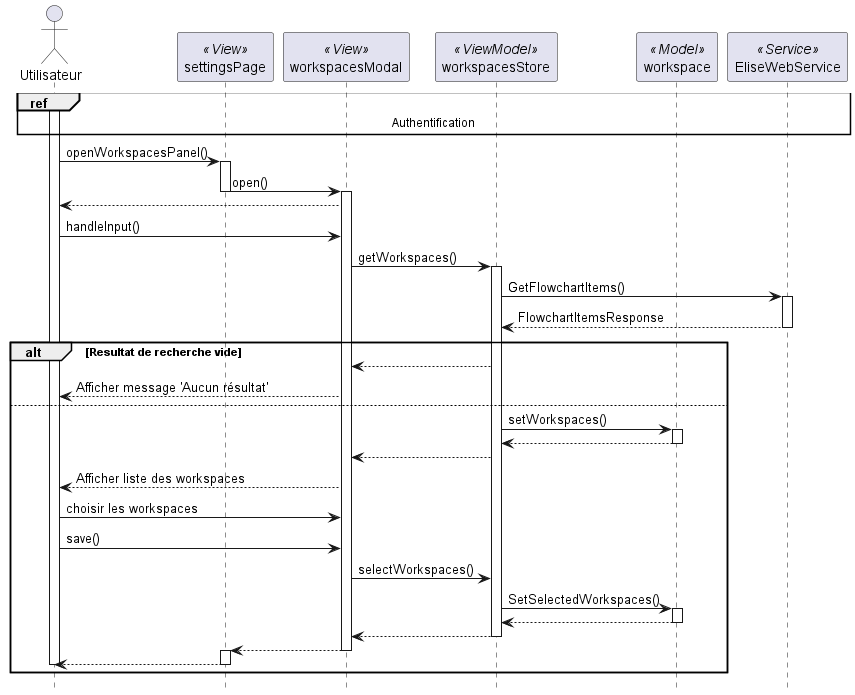
\includegraphics[width=1\textwidth]{out/diagrams/sprint6/sequence_lister_selectionner_workspaces/sequence_lister_selectionner_workspaces}
  \caption{Diagramme de séquence de conception de cas d'utilisation « Lister et sélectionner les espaces de travail »}
  \label{fig:conception_sequence_lister_selectionner_workspaces}
\end{figure}

\begin{figure}[H]
  \centering
  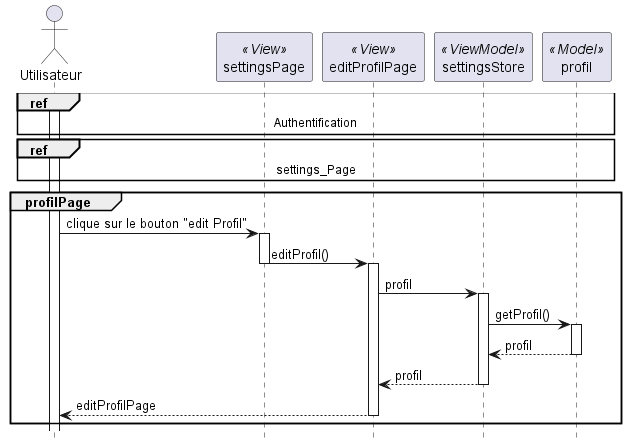
\includegraphics[width=1\textwidth]{out/diagrams/sprint6/sequence_visualiser_profil/sequence_visualiser_profil}
  \caption{Diagramme de séquence de conception de cas d'utilisation «  Visualiser les informations personnelles »}
  \label{fig:conception_sequence_visualiser_profil}
\end{figure}

\begin{figure}[H]
  \centering
  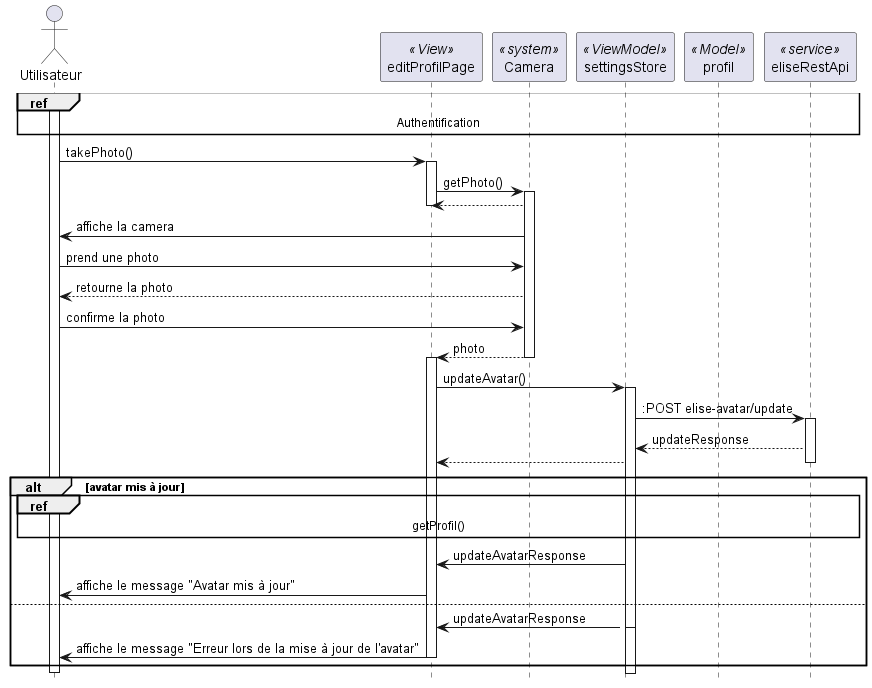
\includegraphics[width=1\textwidth]{out/diagrams/sprint6/sequence_edit_profil_avatar/sequence_edit_profil_avatar}
  \caption{Diagramme de séquence de conception de cas d'utilisation «  Modifier la photo de profil »}
  \label{fig:conception_sequence_edit_profil_avatar}
\end{figure}

\begin{figure}[H]
  \centering
  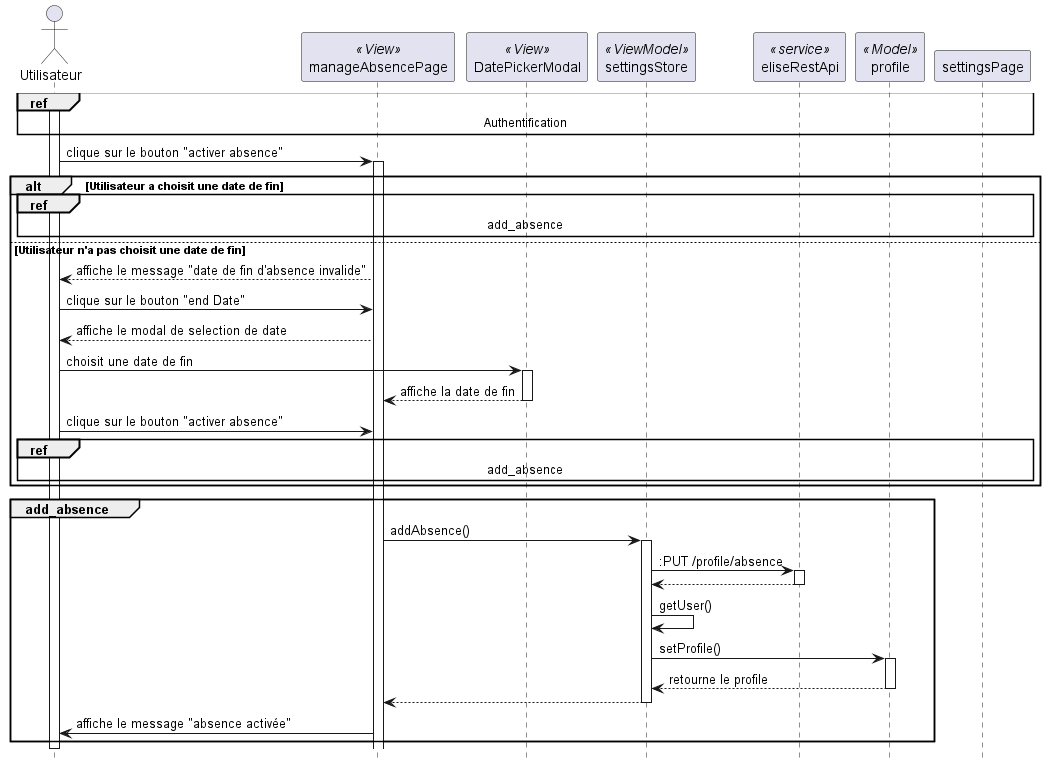
\includegraphics[width=1\textwidth]{out/diagrams/sprint6/sequence_declare_absence/sequence_declare_absence}
  \caption{Diagramme de séquence de conception de cas d'utilisation «  Déclarer l'absence »}
  \label{fig:conception_sequence_declare_absence}
\end{figure}

\begin{figure}[H]
  \centering
  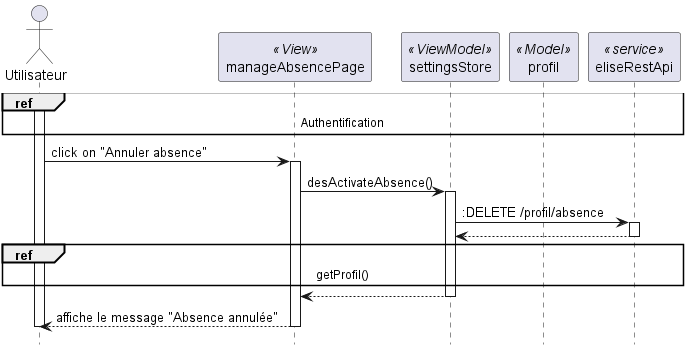
\includegraphics[width=1\textwidth]{out/diagrams/sprint6/sequence_annuler_absence/sequence_annuler_absence}
  \caption{Diagramme de séquence de conception de cas d'utilisation « Annuler une déclaration d'absence »}
  \label{fig:conception_sequence_annuler_absence}
\end{figure}

\begin{figure}[H]
  \centering
  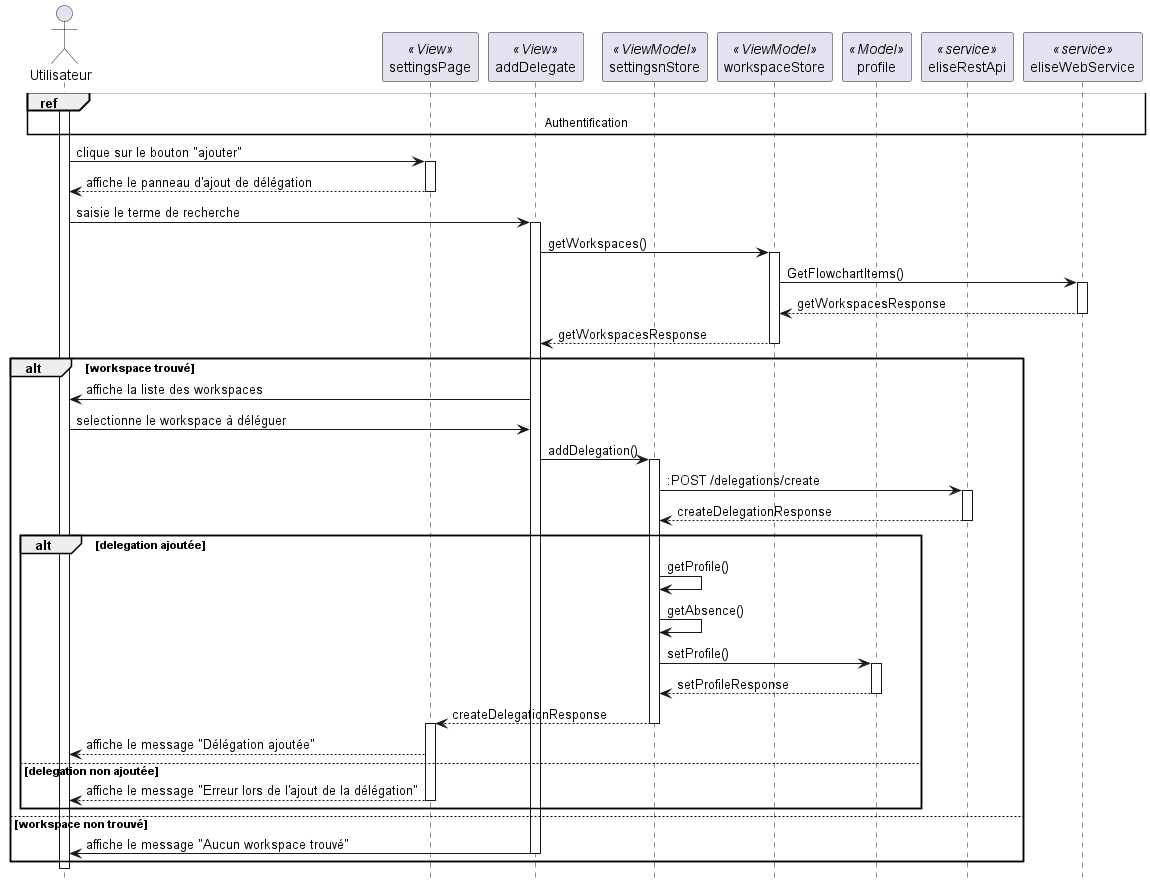
\includegraphics[width=1\textwidth]{out/diagrams/sprint6/sequence_search_affect_delegation/sequence_search_affect_delegation}
  \caption{Diagramme de séquence de conception de cas d'utilisation «  Rechercher et affecter un délégué »}
  \label{fig:conception_sequence_search_affect_delegation}
\end{figure}

\begin{figure}[H]
  \centering
  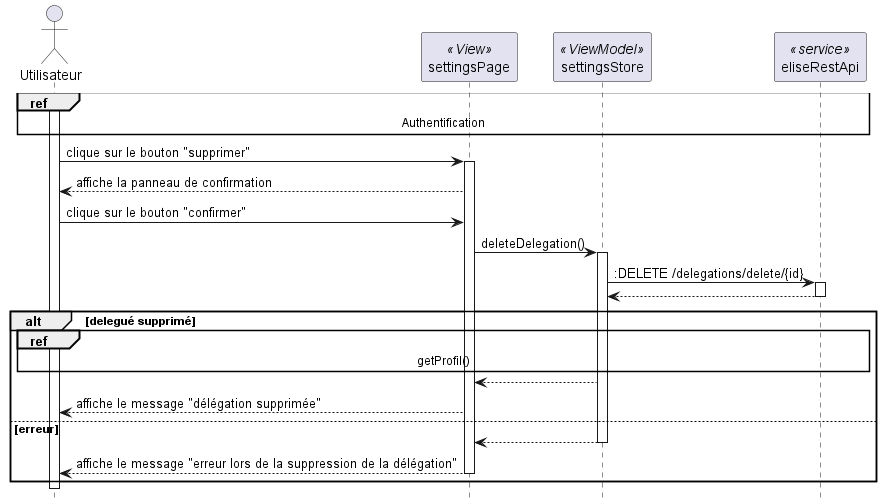
\includegraphics[width=1\textwidth]{out/diagrams/sprint6/sequence_annulation_delegation/sequence_annulation_delegation}
  \caption{Diagramme de séquence de conception de cas d'utilisation « Supprimer un délégué »}
  \label{fig:conception_sequence_annulation_delegation}
\end{figure}




\subsubsection{Réalisation}

Après la présentation des diagrammes d'analyse, nous avons présenté dans cette partie des captures d'écran de l'application.
\begin{figure}[H]
  \centering
  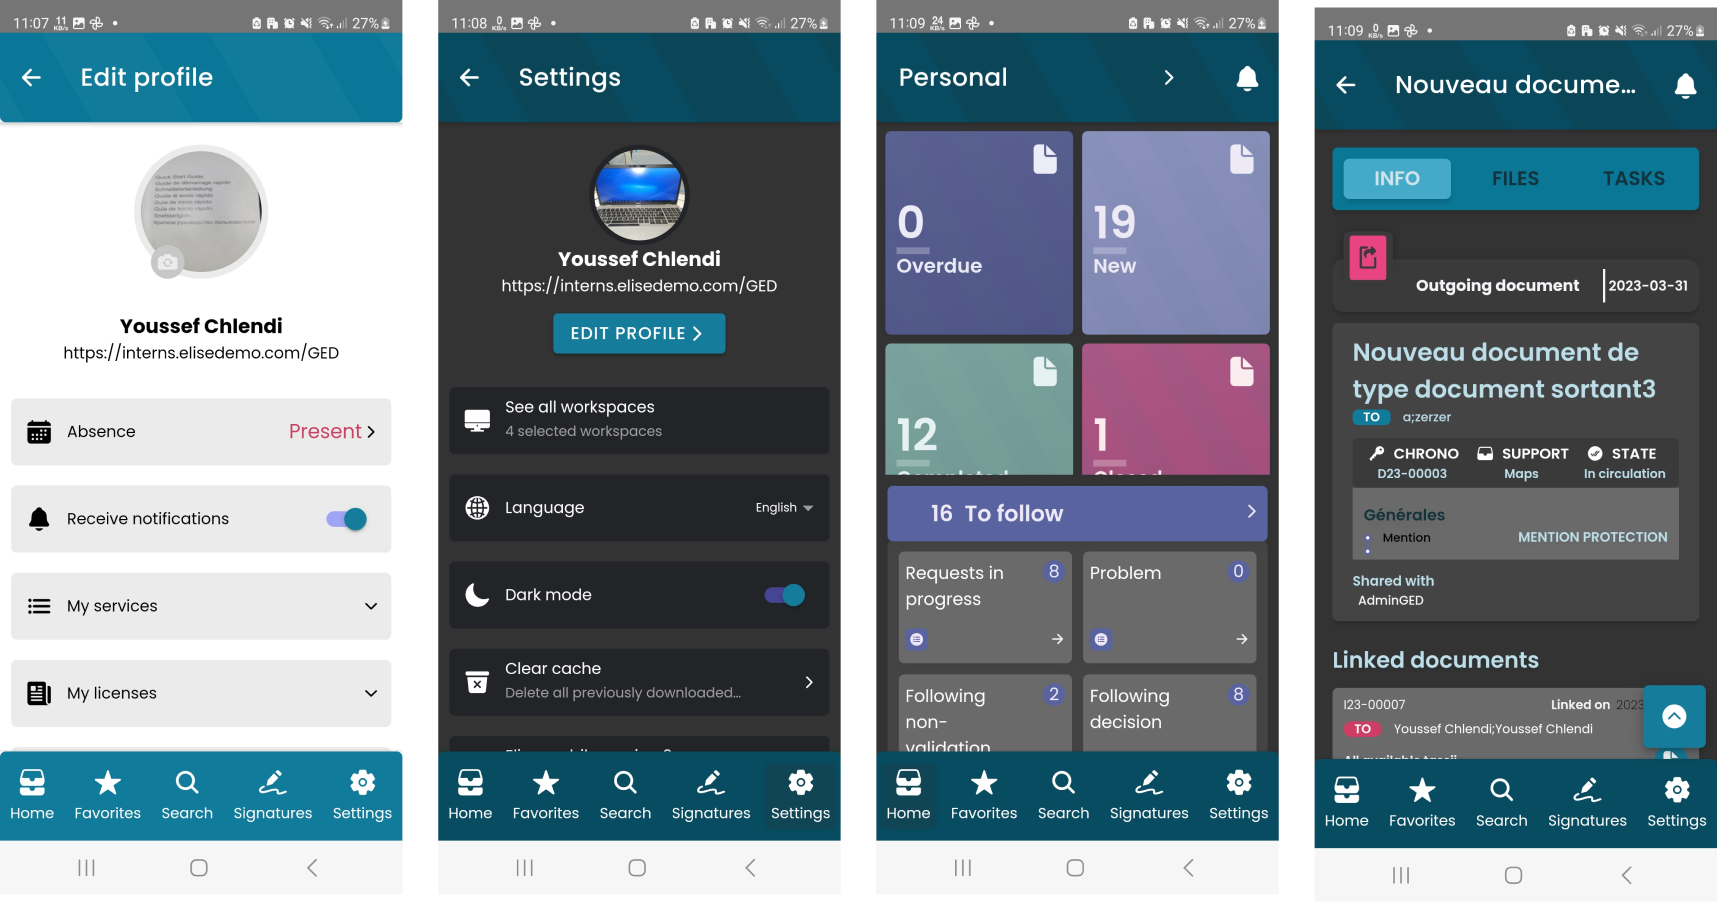
\includegraphics[width=0.7\textwidth]{realisation_sprint61}
  \caption{Realisation de l'interface de paramétrage de l'application et la mode sombre}
  \label{fig:RealisationInterfaceParametrage}
\end{figure}

\begin{figure}[H]
  \centering
  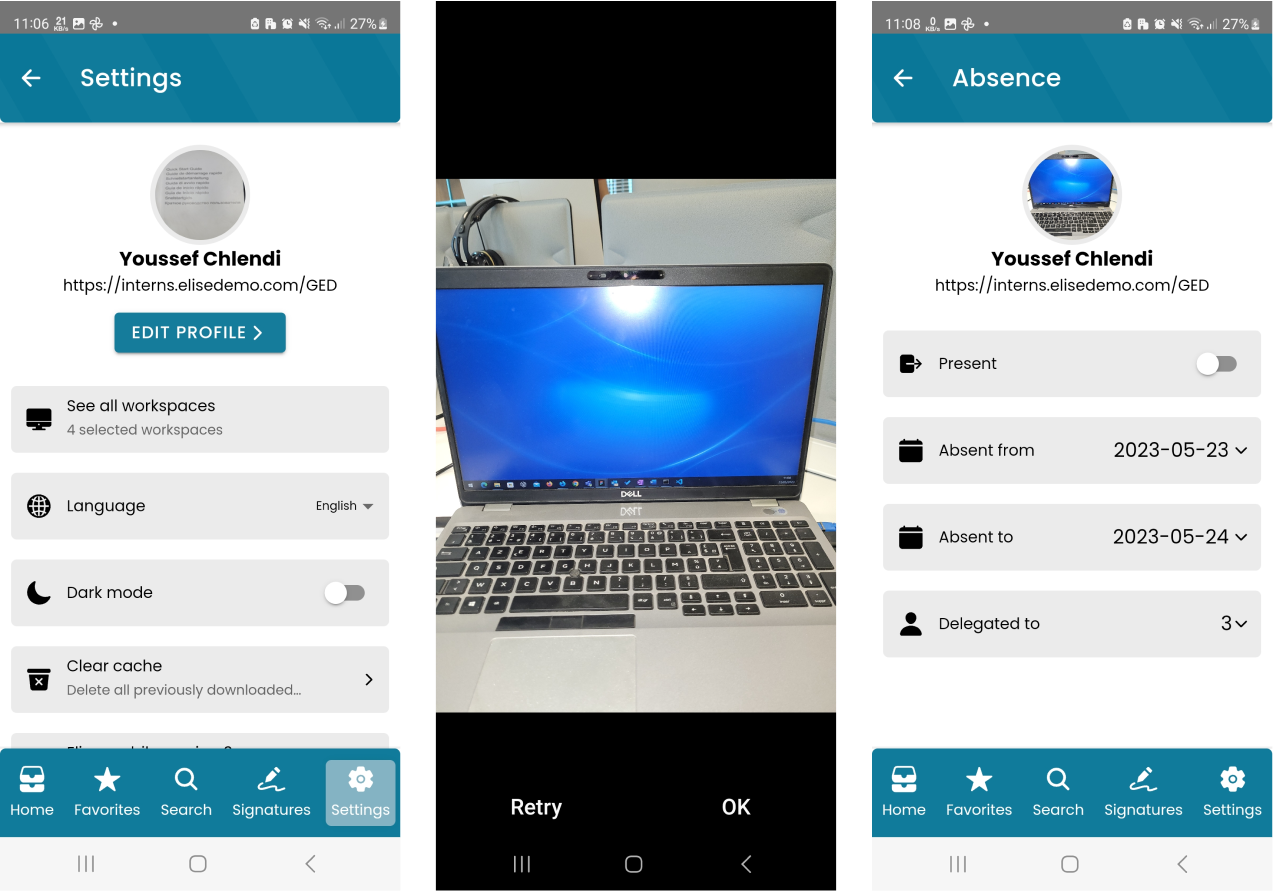
\includegraphics[width=0.7\textwidth]{realisation_sprint62}
  \caption{Realisation de l'interface de modification de profil et gestion d'absence}
  \label{fig:RealisationInterfaceModificationProfil}
\end{figure}

\subsection{Sprint Review}
Dans ce sprint, nous avons implémenté les fonctionnalités suivantes :
\begin{itemize}
  \item \textbf{Paramétrage de l'application :} Nous avons implémenté le paramétrage de l'application dans l'application Elise Mobile, qui permet aux utilisateurs de modifier les paramètres de l'application, tels que la langue, le mode sombre, etc.\\
  \item \textbf{Gestion des absences :} Nous avons implémenté la gestion des absences dans l'application Elise Mobile, qui permet aux utilisateurs de consulter leurs absences et de créer une nouvelle demande d'absence.\\
\end{itemize}
\subsection{Sprint Retrospective}
Nous avons atteint tous les objectifs fixés pour ce sprint :
\begin{itemize}
  \item \textbf{Ce qui a bien fonctionné :}
  \begin{itemize}
    \item L'integration de l'api rest dans l'application Elise Mobile,
    \item L'ajout de la mode sombre dans l'application Elise Mobile,
  \end{itemize}

    \item \textbf{Ce qui n'a pas bien fonctionné :}
    \begin{itemize}
      \item L'ajout de la fonctionnalité de multi-langue dans l'application Elise Mobile dans la deuxième release n'etait pas assez flexible car il faut reécrire tout l'ancien code pour l'adapter avec la nouvelle fonctionnalité.
    \end{itemize}
      
\end{itemize}
\section{Sprint 7 (Consultation des statistique)}

\subsection{Sprint Goal}
L'objectif de ce sprint est de permettre à l'utilisateur de consulter les statistiques de ses documents et consulter les documents a l'aide de filtre rapide de statistique.

\subsection{Sprint Backlog}


\begin{adjustwidth}{-1cm}{}
  % \usepackage{longtable}
    
    \begin{longtable}{|c|p{6cm}|c|p{6cm}|c|}
      % \centering
      \hline
      \textbf{ID} & \textbf{User story} & \textbf{ID}  & \textbf{Tâche} & \textbf{Durée} \\
      \hline
      \multirow{2}{*}{1} & En tant qu'utilisateur, je veux visualiser les statistiques de l'application afin de suivre l'évolution de l'application.
      & 1.1 & Préparer les interfaces sur Figma. & \multirow{3}{*}{2.5 Jour} \\
      \cline{3-4}
      & & 1.2 & Développer le composant de statistique a une valeur. & \\
      \cline{3-4}
      & & 1.3 & Développer le composant de statistique a plusieurs valeurs. & \\
      \cline{3-4}
      & & 1.4 & Développer la fonction qui recuperer et ranger les statistiques. & \\
      & & 1.5 & Développer la fonction qui permet de visualiser les statistiques. & \\
      % & & 1.6 & Développer la fonction qui permet de filtrer les documents par statistique. & \\
      \cline{1-5}

      \multirow{2}{*}{2} & En tant qu'utilisateur, je veux basculer entre mes espaces de travail selectionné a fin de consulter les differents statistiques. & 2.1.& Préparer l'interface sur figma. & \multirow{2}{*}{0.5 Jour} \\
      \cline{3-4}
      & &  2.2 & Développer la fonction qui permet de basculer entre les espaces de travail. & \\
      \cline{1-5}
      \multirow{2}{*}{3} & En tant qu'utilisateur, je veux consulter les documents a l'aide de filtre rapide afin de trouver les documents que je cherche. & 3.1.& Ajouter la fonction de filtre a l'interface de consultation des statistiques. & \multirow{2}{*}{0.5 Jour} \\
      \cline{3-4}
      & & 3.2 & Développer la fonction qui permet de filtrer les documents par statistique. & \\
      \cline{1-5}
      \multirow{2}{*}{4} & En tant qu'utilisateur, je veux refraichir les données de l'application afin de voir les dernières informations. & 4.1.& Ajouter l'interface de rafraichissement des données a chaque page possible. & \multirow{2}{*}{0.5 Jour} \\
      \cline{3-4}
      & & 4.2 & Développer la fonction qui permet de rafraichir les données de chaque page. & \\
      \cline{1-5}
  \hline
  \caption{Sprint backlog du Sprint 7}
  \label{tab:sprint-backlog-7}
\end{longtable}
\end{adjustwidth}


\subsection{Implémentation du Sprint 7}
\textbf{•	Diagramme de cas d'utilisation du sprint 7}

% add image
\begin{figure}[H]
  \centering
  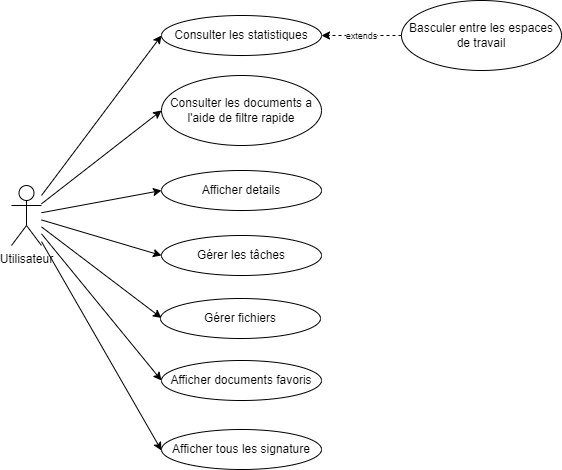
\includegraphics[width=0.6\textwidth]{use_case_sprint_7}
  \caption{Diagramme de cas d'utilisation du sprint 7}
  \label{fig:UseCaseDiagramSp71}
\end{figure}

\subsubsection{Analyse des besoins:}
\textbf{•	Description textuelle de cas d'utilisation « Consulter les statistiques »}

\begin{longtable}{|p{5cm}|p{10cm}|}
\hline
\textbf{Cas d'utilisation}&Consulter les statistiques\\
\hline
\textbf{Acteurs}&Utilisateur\\
\hline
\textbf{Pré Condition}&L'utilisateur est authentifié\\
\hline
\textbf{Post Condition}&Consultation des statistiques\\
\hline
\textbf{Scénario Nominal}&
\vspace{-\baselineskip}
\begin{enumerate}
  \setcounter{enumi}{1}
      \item L'utilisateur clique sur le bouton « Accueil »
      \item  Le système affiche les statistiques
\end{enumerate}\\
\hline
\textbf{Scénario d'exception}&Erreur de connexion\\
\hline
\caption{Description textuelle du diagramme de cas d'utilisation « Consulter les statistiques »}
\label{tab:use_case_consulter_statistiques}
\end{longtable}

\textbf{•	Description textuelle de cas d'utilisation «Basculer entre les espaces de travail »}

\begin{longtable}{|p{5cm}|p{10cm}|}
  \hline
  \textbf{Cas d'utilisation}&Basculer entre les espaces de travail\\
  \hline
  \textbf{Acteurs}&Utilisateur\\
  \hline
  \textbf{Pré Condition}&L'utilisateur selectionne au moins un espace de travail dans la page des paramètres\\
  \hline
  \textbf{Post Condition}&L'utilisateur bascule entre les espaces de travail\\
  \hline
  \textbf{Scénario Nominal}&
  \vspace{-\baselineskip}
  \begin{enumerate}
    \setcounter{enumi}{1}
        \item L'utilisateur clique sur le bouton a coté du nom de l'espace de travail dans la page d'accueil
        \item Le système affiche la liste des espaces de travail selectionnés
        \item L'utilisateur clique sur l'espace de travail qu'il veut utiliser
        \item Le système récupère les données de l'espace de travail selectionné
  \end{enumerate}\\
  \hline
  \textbf{Scénario d'exception}&Erreur de connexion\\
  \hline
  \caption{Description textuelle du diagramme de cas d'utilisation « Basculer entre les espaces de travail »}
  \label{tab:use_case_basculer_espaces_travail}
  \end{longtable}


\textbf{•	Description textuelle de cas d'utilisation « Consulter les documents a l'aide de filtre rapide »}

\begin{longtable}{|p{5cm}|p{10cm}|}
\hline
\textbf{Cas d'utilisation}&Consulter les documents a l'aide de filtre rapide\\
\hline
\textbf{Acteurs}&Utilisateur \\
\hline
\textbf{Pré Condition}&L'utilisateur doit être authentifié\\
\hline
\textbf{Post Condition}&Consultation des documents a l'aide de filtre rapide\\
\hline
\textbf{Scénario Nominal}&
\vspace{-\baselineskip}
\begin{enumerate}
    \setcounter{enumi}{1}
      \item L'utilisateur clique sur l'une des widget
      \item Le système affiche les documents correspondant au filtre
\end{enumerate}\\
\hline
\textbf{Scénario d'exception}&Erreur de connexion\\
\hline
\caption{Description textuelle du diagramme de cas d'utilisation « Consulter les documents a l'aide de filtre rapide »}
\label{tab:use_case_consulter_documents_filtre_rapide}
\end{longtable}

\textbf{•	Description textuelle de cas d'utilisation « Refraichissement
des données »}

% Note:
\textbf{Note: Cette fonctionnalité est disponible sur la page d'accueil, la page de consultation des documents favoris, la page de consultation d'un document et la page des signatures, mais pour des raisons de lisibilité, nous avons choisi de ne pas répéter la description textuelle de ce cas d'utilisation.}

\begin{longtable}{|p{5cm}|p{10cm}|}
\hline
\textbf{Cas d'utilisation}&Refraichissement des données\\
\hline
\textbf{Acteurs}&Utilisateur \\
\hline
\textbf{Pré Condition}&L'utilisateur doit être authentifié\\
\hline
\textbf{Post Condition}&Refraichissement des données\\
\hline
\textbf{Scénario Nominal}&
\vspace{-\baselineskip}
\begin{enumerate}
    \setcounter{enumi}{1}
      \item L'utilisateur glisse son doigt vers le bas sur l'écran
      \item Le système affiche les dernières données
\end{enumerate}\\
\hline
\textbf{Scénario d'exception}&Erreur de connexion\\
\hline
\caption{Description textuelle du diagramme de cas d'utilisation « Refraichissement des données »}
\label{tab:use_case_refraichissement_donnees}
\end{longtable}

\begin{figure}[H]
  \centering
  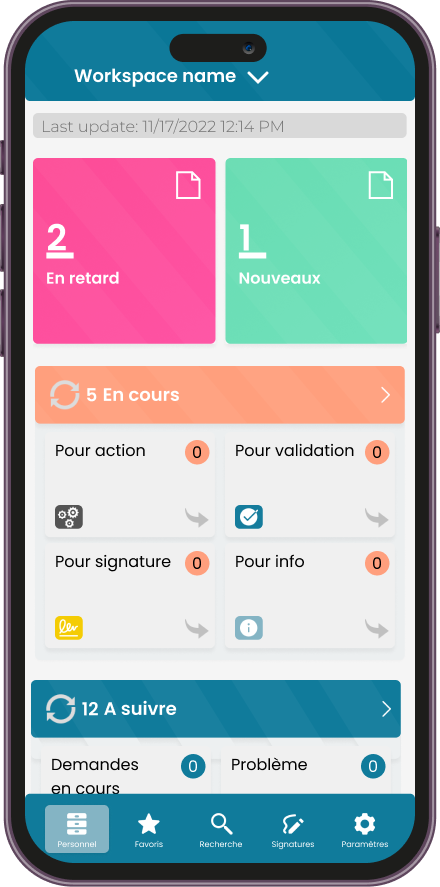
\includegraphics[width=0.5\textwidth]{design_statistique}
  \caption{Maquette de la page de statistique et choix d'espace de travail}
  \label{fig:design_statistique}
\end{figure}


Pour avoir une représentation temporelle des interactions entre les objets de notre système et de la chronologie des messages échangés entre eux et avec les acteurs nous avons réalisé les diagrammes de séquence représentés ci-dessous

\begin{figure}[H]
  \centering
  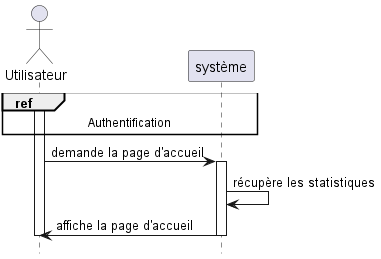
\includegraphics[width=0.7\textwidth]{out/diagrams/sprint7/view_stats/view_stats}
  \caption{Diagramme de séquence de cas d'utilisation « Consulter les statistiques »}
  \label{fig:sequence_view_stats}
\end{figure}

\begin{figure}[H]
  \centering
  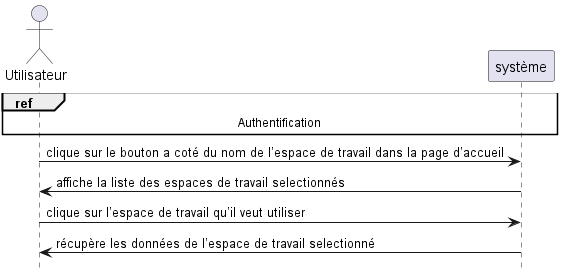
\includegraphics[width=0.7\textwidth]{out/diagrams/sprint7/switch_workspace/switch_workspace}
  \caption{Diagramme de séquence de cas d'utilisation « Basculer entre les espaces de travail »}
  \label{fig:sequence_switch_workspace}
\end{figure}

\begin{figure}[H]
  \centering
  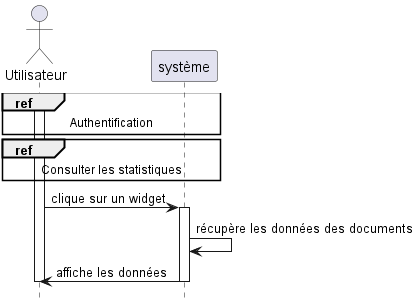
\includegraphics[width=0.7\textwidth]{out/diagrams/sprint7/docs_quick_filter/docs_quick_filter}
  \caption{Diagramme de séquence de cas d'utilisation « Consulter les documents a l'aide de filtre rapide »}
  \label{fig:sequence_docs_quick_filter}
\end{figure}

\textbf{Note: Cette fonctionnalité est disponible sur la page d'accueil, la page de consultation des documents favoris, la page de consultation d'un document et la page des signatures, mais pour des raisons de lisibilité, nous avons choisi de ne pas répéter le diagramme de séquence de ce cas d'utilisation.}
\begin{figure}[H]
  \centering
  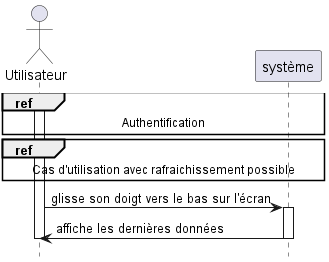
\includegraphics[width=0.7\textwidth]{out/diagrams/sprint7/refresh_data/refresh_data}
  \caption{Diagramme de séquence de cas d'utilisation « Refraichissement des données »}
  \label{fig:sequence_refresh_data}
\end{figure}


\subsubsection{Analyse détaillée}
La présentation de démarche d'analyse fonctionnelle d'un sprint est très importante pour la satisfaction d'un client parce qu'elle consiste à caractériser les fonctions offertes par un produit.
Donc, nous allons faire l'analyse des différents cas d'utilisation en utilisant le diagramme de classes d'analyse.


% spacing between paragraphs
\setlength{\parskip}{1em}
% spacing left
\setlength{\parindent}{0em}

\textbf{•	Diagramme de classe d'analyse de sprint 7 }


\begin{figure}[H]
  \centering
  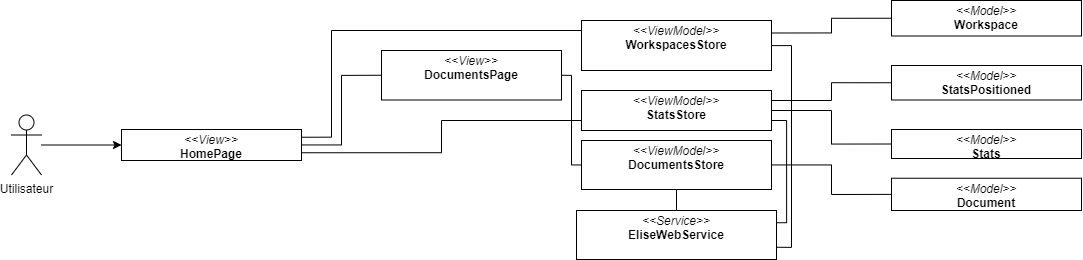
\includegraphics[width=1\textwidth]{dca_sprint7}
  \caption{Diagramme de classe d'analyse de sprint 7}
  \label{fig:class_analyse_sprint7}
\end{figure}


\subsubsection{Conception}

Après la présentation des diagrammes d'analyse, nous avons présenté dans cette partie les diagrammes de conception.\\ 
Nous allons présenter dans cette partie les diagrammes de conception de sprint 7. \\
\begin{landscape}

\textbf{•	Diagramme de classe de conception de sprint 7}

% add image
\begin{figure}[H]
  \centering
  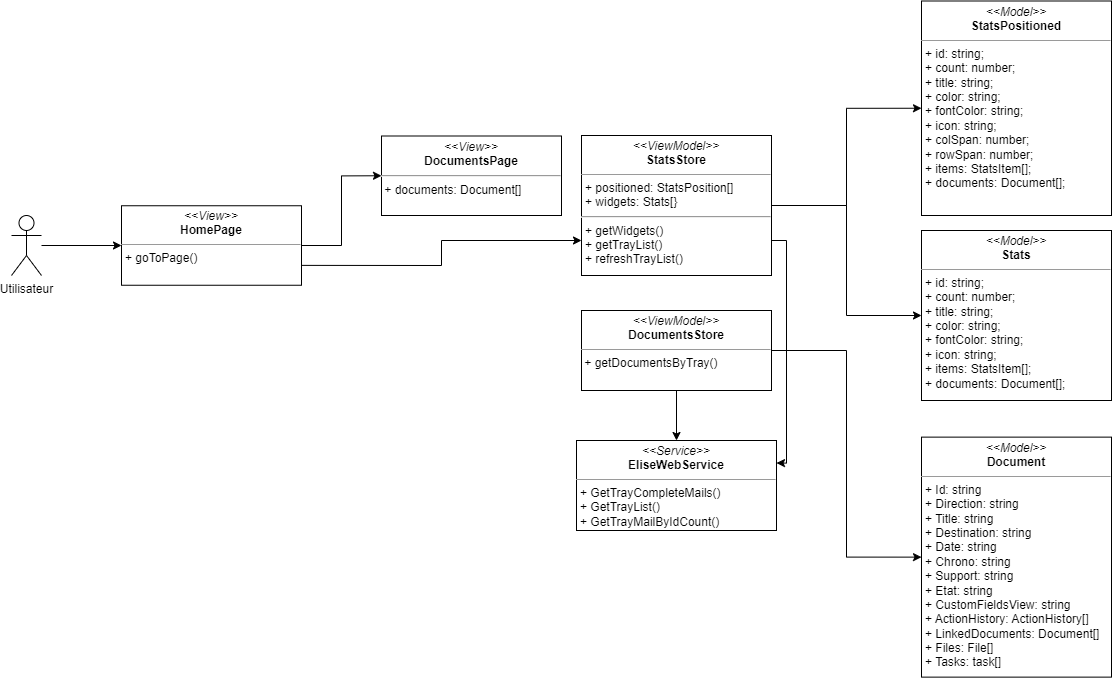
\includegraphics[width=1\textwidth]{dcc_sprint7}
  \caption{Diagramme de classe de conception de sprint 7}
  \label{fig:class_diagram_5}
\end{figure}
\end{landscape}


\begin{figure}[H]
  \centering
  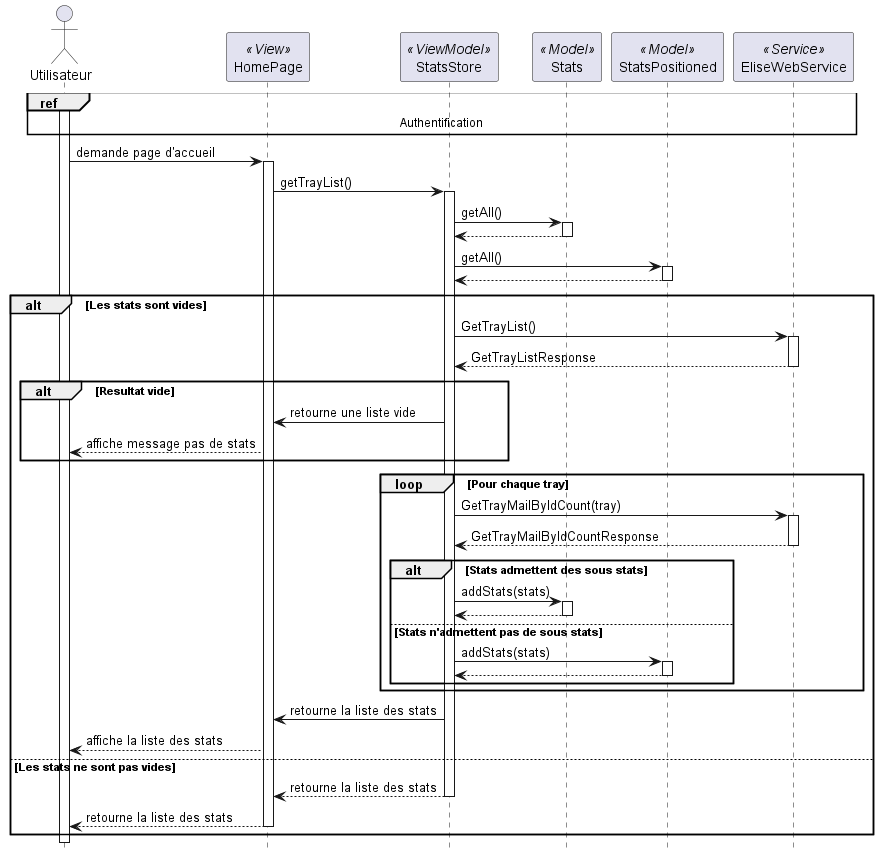
\includegraphics[width=1\textwidth]{out/diagrams/sprint7/sequence_view_stats/sequence_view_stats}
  \caption{Diagramme de séquence de conception de cas d'utilisation « Consulter les statistiques »}
  \label{fig:sequence_conception_consulter_statistiques}
\end{figure}

\begin{figure}[H]
  \centering
  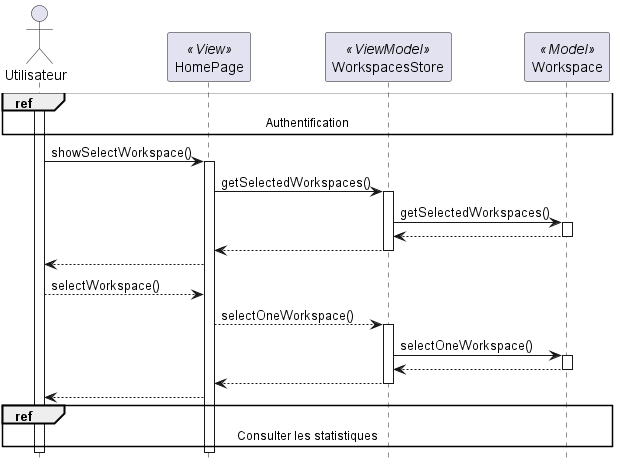
\includegraphics[width=1\textwidth]{out/diagrams/sprint7/sequence_switch_workspace/sequence_switch_workspace}
  \caption{Diagramme de séquence de conception de cas d'utilisation « Basculer entre les espaces de travail »}
  \label{fig:sequence_conception_sequence_switch_workspace}
\end{figure}


\begin{figure}[H]
  \centering
  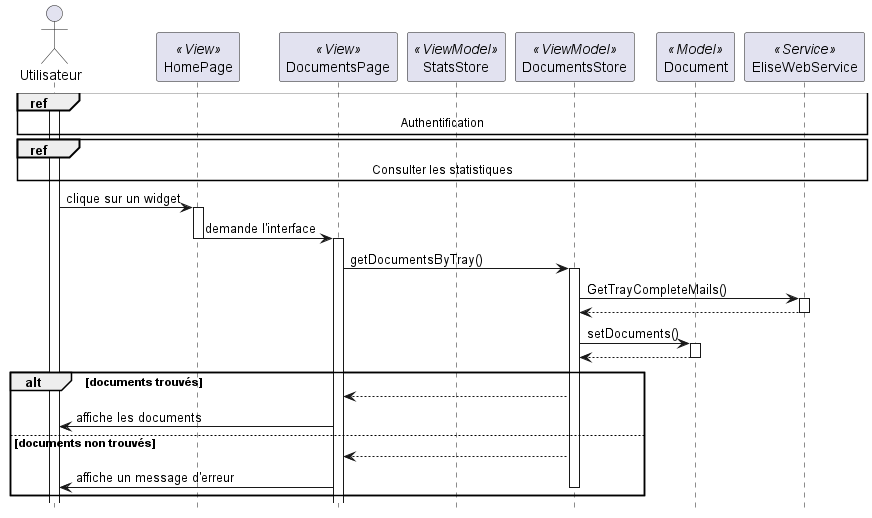
\includegraphics[width=1\textwidth]{out/diagrams/sprint7/sequence_docs_quick_filter/sequence_docs_quick_filter}
  \caption{Diagramme de séquence de conception de cas d'utilisation « Consulter les documents a l'aide de filtre rapide »}
  \label{fig:sequence_conception_consulter_documents_filtre_rapide}
\end{figure}

\begin{figure}[H]
  \centering
  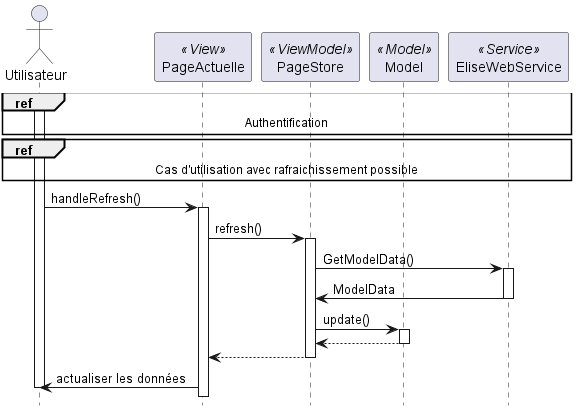
\includegraphics[width=1\textwidth]{out/diagrams/sprint7/sequence_refresh_data/sequence_refresh_data}
  \caption{Diagramme de séquence de conception de cas d'utilisation « Refraichissement des données »}
  \label{fig:sequence_conception_refraichissement_donnees}
\end{figure}
\textbf{Note: Cette fonctionnalité est disponible sur la page d'accueil, la page de consultation des documents favoris, la page de consultation d'un document et la page des signatures, mais pour des raisons de lisibilité, nous avons choisi de ne pas répéter le diagramme de séquence de ce cas d'utilisation.}

\subsubsection{Réalisation}

Après la présentation des diagrammes d'analyse, nous avons présenté dans cette partie des captures d'écran de l'application.

% add image
\begin{figure}[H]
  \centering
  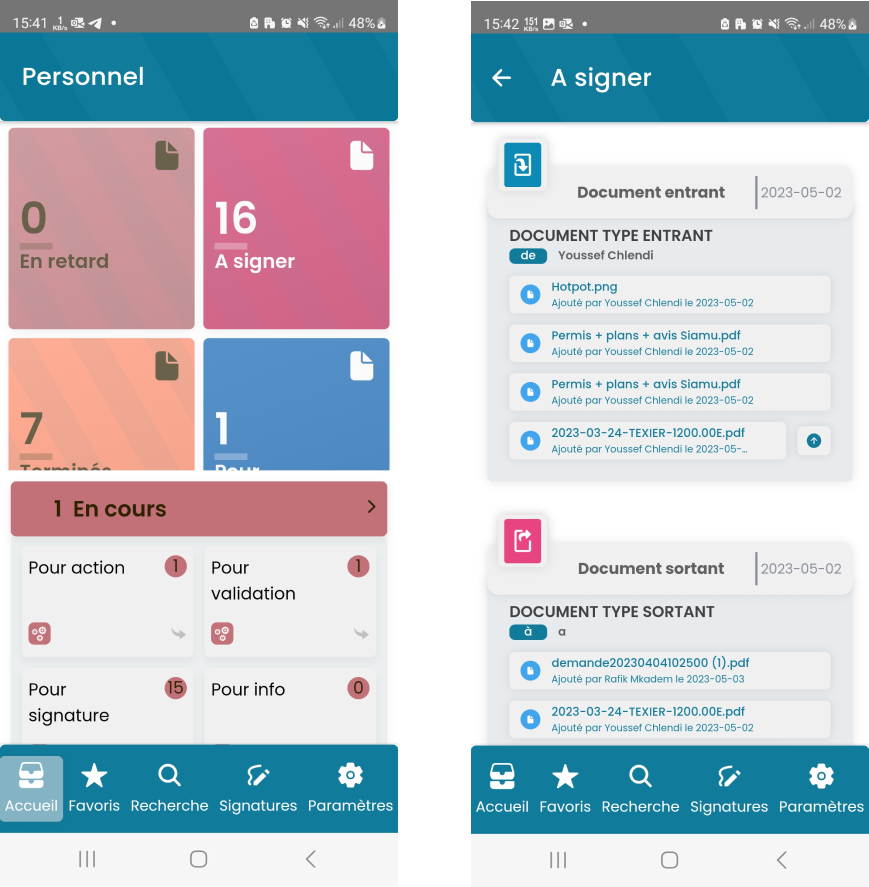
\includegraphics[width=0.7\textwidth, height=0.7\textheight,keepaspectratio=true]{realisation_sprint7}
  \caption{Les interfaces de consultation des statistiques et des documents à l'aide de filtre rapide}
  \label{fig:realisation_sprint7}
\end{figure}

\subsection{Sprint Review}
Suite à cette Technical Story, nous avons pu réaliser les fonctionnalités suivantes :
\begin{itemize}
  \item \textbf{Consulter les statistiques :} Cette fonctionnalité permet à l'utilisateur de consulter les statistiques des documents et des signatures.
  \item \textbf{Basculer entre les espaces de travail :} Cette fonctionnalité permet à l'utilisateur de basculer entre les espaces de travail.
  \item \textbf{Consulter les documents à l'aide de filtre rapide :} Cette fonctionnalité permet à l'utilisateur de consulter les documents à l'aide de filtre rapide.
  \item \textbf{Rafraichissement des données :} Cette fonctionnalité permet à l'utilisateur de rafraichir les données.
\end{itemize}

\subsection{Sprint Retrospective}

\begin{itemize}
  \item \textbf{Ce qui a bien fonctionné :}
  \begin{itemize}
    \item Nous avons pu réaliser toutes les fonctionnalités prévues pour ce sprint.
  \end{itemize}

    \item \textbf{Ce qui n'a pas bien fonctionné :}
    \begin{itemize}
      \item Nous avons eu des difficultés à réaliser la fonctionnalité de consultation des statistiques.
    \end{itemize}
      
\end{itemize}
